% Options for packages loaded elsewhere
\PassOptionsToPackage{unicode}{hyperref}
\PassOptionsToPackage{hyphens}{url}
\PassOptionsToPackage{dvipsnames,svgnames,x11names}{xcolor}
%
\documentclass[
  letterpaper,
  DIV=11,
  numbers=noendperiod]{scrreprt}

\usepackage{amsmath,amssymb}
\usepackage{lmodern}
\usepackage{iftex}
\ifPDFTeX
  \usepackage[T1]{fontenc}
  \usepackage[utf8]{inputenc}
  \usepackage{textcomp} % provide euro and other symbols
\else % if luatex or xetex
  \usepackage{unicode-math}
  \defaultfontfeatures{Scale=MatchLowercase}
  \defaultfontfeatures[\rmfamily]{Ligatures=TeX,Scale=1}
\fi
% Use upquote if available, for straight quotes in verbatim environments
\IfFileExists{upquote.sty}{\usepackage{upquote}}{}
\IfFileExists{microtype.sty}{% use microtype if available
  \usepackage[]{microtype}
  \UseMicrotypeSet[protrusion]{basicmath} % disable protrusion for tt fonts
}{}
\makeatletter
\@ifundefined{KOMAClassName}{% if non-KOMA class
  \IfFileExists{parskip.sty}{%
    \usepackage{parskip}
  }{% else
    \setlength{\parindent}{0pt}
    \setlength{\parskip}{6pt plus 2pt minus 1pt}}
}{% if KOMA class
  \KOMAoptions{parskip=half}}
\makeatother
\usepackage{xcolor}
\setlength{\emergencystretch}{3em} % prevent overfull lines
\setcounter{secnumdepth}{5}
% Make \paragraph and \subparagraph free-standing
\ifx\paragraph\undefined\else
  \let\oldparagraph\paragraph
  \renewcommand{\paragraph}[1]{\oldparagraph{#1}\mbox{}}
\fi
\ifx\subparagraph\undefined\else
  \let\oldsubparagraph\subparagraph
  \renewcommand{\subparagraph}[1]{\oldsubparagraph{#1}\mbox{}}
\fi

\usepackage{color}
\usepackage{fancyvrb}
\newcommand{\VerbBar}{|}
\newcommand{\VERB}{\Verb[commandchars=\\\{\}]}
\DefineVerbatimEnvironment{Highlighting}{Verbatim}{commandchars=\\\{\}}
% Add ',fontsize=\small' for more characters per line
\usepackage{framed}
\definecolor{shadecolor}{RGB}{241,243,245}
\newenvironment{Shaded}{\begin{snugshade}}{\end{snugshade}}
\newcommand{\AlertTok}[1]{\textcolor[rgb]{0.68,0.00,0.00}{#1}}
\newcommand{\AnnotationTok}[1]{\textcolor[rgb]{0.37,0.37,0.37}{#1}}
\newcommand{\AttributeTok}[1]{\textcolor[rgb]{0.40,0.45,0.13}{#1}}
\newcommand{\BaseNTok}[1]{\textcolor[rgb]{0.68,0.00,0.00}{#1}}
\newcommand{\BuiltInTok}[1]{\textcolor[rgb]{0.00,0.23,0.31}{#1}}
\newcommand{\CharTok}[1]{\textcolor[rgb]{0.13,0.47,0.30}{#1}}
\newcommand{\CommentTok}[1]{\textcolor[rgb]{0.37,0.37,0.37}{#1}}
\newcommand{\CommentVarTok}[1]{\textcolor[rgb]{0.37,0.37,0.37}{\textit{#1}}}
\newcommand{\ConstantTok}[1]{\textcolor[rgb]{0.56,0.35,0.01}{#1}}
\newcommand{\ControlFlowTok}[1]{\textcolor[rgb]{0.00,0.23,0.31}{#1}}
\newcommand{\DataTypeTok}[1]{\textcolor[rgb]{0.68,0.00,0.00}{#1}}
\newcommand{\DecValTok}[1]{\textcolor[rgb]{0.68,0.00,0.00}{#1}}
\newcommand{\DocumentationTok}[1]{\textcolor[rgb]{0.37,0.37,0.37}{\textit{#1}}}
\newcommand{\ErrorTok}[1]{\textcolor[rgb]{0.68,0.00,0.00}{#1}}
\newcommand{\ExtensionTok}[1]{\textcolor[rgb]{0.00,0.23,0.31}{#1}}
\newcommand{\FloatTok}[1]{\textcolor[rgb]{0.68,0.00,0.00}{#1}}
\newcommand{\FunctionTok}[1]{\textcolor[rgb]{0.28,0.35,0.67}{#1}}
\newcommand{\ImportTok}[1]{\textcolor[rgb]{0.00,0.46,0.62}{#1}}
\newcommand{\InformationTok}[1]{\textcolor[rgb]{0.37,0.37,0.37}{#1}}
\newcommand{\KeywordTok}[1]{\textcolor[rgb]{0.00,0.23,0.31}{#1}}
\newcommand{\NormalTok}[1]{\textcolor[rgb]{0.00,0.23,0.31}{#1}}
\newcommand{\OperatorTok}[1]{\textcolor[rgb]{0.37,0.37,0.37}{#1}}
\newcommand{\OtherTok}[1]{\textcolor[rgb]{0.00,0.23,0.31}{#1}}
\newcommand{\PreprocessorTok}[1]{\textcolor[rgb]{0.68,0.00,0.00}{#1}}
\newcommand{\RegionMarkerTok}[1]{\textcolor[rgb]{0.00,0.23,0.31}{#1}}
\newcommand{\SpecialCharTok}[1]{\textcolor[rgb]{0.37,0.37,0.37}{#1}}
\newcommand{\SpecialStringTok}[1]{\textcolor[rgb]{0.13,0.47,0.30}{#1}}
\newcommand{\StringTok}[1]{\textcolor[rgb]{0.13,0.47,0.30}{#1}}
\newcommand{\VariableTok}[1]{\textcolor[rgb]{0.07,0.07,0.07}{#1}}
\newcommand{\VerbatimStringTok}[1]{\textcolor[rgb]{0.13,0.47,0.30}{#1}}
\newcommand{\WarningTok}[1]{\textcolor[rgb]{0.37,0.37,0.37}{\textit{#1}}}

\providecommand{\tightlist}{%
  \setlength{\itemsep}{0pt}\setlength{\parskip}{0pt}}\usepackage{longtable,booktabs,array}
\usepackage{calc} % for calculating minipage widths
% Correct order of tables after \paragraph or \subparagraph
\usepackage{etoolbox}
\makeatletter
\patchcmd\longtable{\par}{\if@noskipsec\mbox{}\fi\par}{}{}
\makeatother
% Allow footnotes in longtable head/foot
\IfFileExists{footnotehyper.sty}{\usepackage{footnotehyper}}{\usepackage{footnote}}
\makesavenoteenv{longtable}
\usepackage{graphicx}
\makeatletter
\def\maxwidth{\ifdim\Gin@nat@width>\linewidth\linewidth\else\Gin@nat@width\fi}
\def\maxheight{\ifdim\Gin@nat@height>\textheight\textheight\else\Gin@nat@height\fi}
\makeatother
% Scale images if necessary, so that they will not overflow the page
% margins by default, and it is still possible to overwrite the defaults
% using explicit options in \includegraphics[width, height, ...]{}
\setkeys{Gin}{width=\maxwidth,height=\maxheight,keepaspectratio}
% Set default figure placement to htbp
\makeatletter
\def\fps@figure{htbp}
\makeatother

\KOMAoption{captions}{tableheading}
\makeatletter
\@ifpackageloaded{tcolorbox}{}{\usepackage[many]{tcolorbox}}
\@ifpackageloaded{fontawesome5}{}{\usepackage{fontawesome5}}
\definecolor{quarto-callout-color}{HTML}{909090}
\definecolor{quarto-callout-note-color}{HTML}{0758E5}
\definecolor{quarto-callout-important-color}{HTML}{CC1914}
\definecolor{quarto-callout-warning-color}{HTML}{EB9113}
\definecolor{quarto-callout-tip-color}{HTML}{00A047}
\definecolor{quarto-callout-caution-color}{HTML}{FC5300}
\definecolor{quarto-callout-color-frame}{HTML}{acacac}
\definecolor{quarto-callout-note-color-frame}{HTML}{4582ec}
\definecolor{quarto-callout-important-color-frame}{HTML}{d9534f}
\definecolor{quarto-callout-warning-color-frame}{HTML}{f0ad4e}
\definecolor{quarto-callout-tip-color-frame}{HTML}{02b875}
\definecolor{quarto-callout-caution-color-frame}{HTML}{fd7e14}
\makeatother
\makeatletter
\makeatother
\makeatletter
\makeatother
\makeatletter
\@ifpackageloaded{caption}{}{\usepackage{caption}}
\AtBeginDocument{%
\ifdefined\contentsname
  \renewcommand*\contentsname{Table of contents}
\else
  \newcommand\contentsname{Table of contents}
\fi
\ifdefined\listfigurename
  \renewcommand*\listfigurename{List of Figures}
\else
  \newcommand\listfigurename{List of Figures}
\fi
\ifdefined\listtablename
  \renewcommand*\listtablename{List of Tables}
\else
  \newcommand\listtablename{List of Tables}
\fi
\ifdefined\figurename
  \renewcommand*\figurename{Figure}
\else
  \newcommand\figurename{Figure}
\fi
\ifdefined\tablename
  \renewcommand*\tablename{Table}
\else
  \newcommand\tablename{Table}
\fi
}
\@ifpackageloaded{float}{}{\usepackage{float}}
\floatstyle{ruled}
\@ifundefined{c@chapter}{\newfloat{codelisting}{h}{lop}}{\newfloat{codelisting}{h}{lop}[chapter]}
\floatname{codelisting}{Listing}
\newcommand*\listoflistings{\listof{codelisting}{List of Listings}}
\makeatother
\makeatletter
\@ifpackageloaded{caption}{}{\usepackage{caption}}
\@ifpackageloaded{subcaption}{}{\usepackage{subcaption}}
\makeatother
\makeatletter
\@ifpackageloaded{tcolorbox}{}{\usepackage[many]{tcolorbox}}
\makeatother
\makeatletter
\@ifundefined{shadecolor}{\definecolor{shadecolor}{rgb}{.97, .97, .97}}
\makeatother
\makeatletter
\makeatother
\ifLuaTeX
  \usepackage{selnolig}  % disable illegal ligatures
\fi
\IfFileExists{bookmark.sty}{\usepackage{bookmark}}{\usepackage{hyperref}}
\IfFileExists{xurl.sty}{\usepackage{xurl}}{} % add URL line breaks if available
\urlstyle{same} % disable monospaced font for URLs
\hypersetup{
  pdftitle={DS 1001 Active Learning Modules},
  pdfauthor={R.C. Alvarado},
  colorlinks=true,
  linkcolor={blue},
  filecolor={Maroon},
  citecolor={Blue},
  urlcolor={Blue},
  pdfcreator={LaTeX via pandoc}}

\title{DS 1001 Active Learning Modules}
\author{R.C. Alvarado}
\date{8/23/23}

\begin{document}
\maketitle
\ifdefined\Shaded\renewenvironment{Shaded}{\begin{tcolorbox}[interior hidden, borderline west={3pt}{0pt}{shadecolor}, sharp corners, boxrule=0pt, breakable, enhanced, frame hidden]}{\end{tcolorbox}}\fi

\renewcommand*\contentsname{Table of contents}
{
\hypersetup{linkcolor=}
\setcounter{tocdepth}{2}
\tableofcontents
}
\part{Preface}

This is a Quarto book.

To learn more about Quarto books visit
\url{https://quarto.org/docs/books}.

\hypertarget{rubric-active-learning-lab-sessions}{%
\chapter{Rubric Active Learning Lab
Sessions}\label{rubric-active-learning-lab-sessions}}

\textbf{Requirements}

\begin{itemize}
\tightlist
\item
  Create three assessments.
\item
  For AY 2023-24.
\item
  Can embedded into undergraduate data science courses.
\item
  Should cover a two-week period.
\item
  Each contains elements described below.
\item
  Assessments are transparent.
\item
  Assessments are authentic.
\end{itemize}

President and Provost's Fund for Institutionally Related Research: Data
Science Active Learning Lab.

\hypertarget{project-description}{%
\section{PROJECT DESCRIPTION}\label{project-description}}

Active learning approaches have not been widely applied and tested in
data science courses despite significant research supporting their
benefits and its successful adoption in computer science. One study
notes a 33\% increase in pass rates for computer science courses
employing active learning as compared to traditional lecture classes
\textsuperscript{{[}3{]}}. The Academy for Teaching Excellence has
thousands of resources to aid in the teaching of computer science
content with hundreds of assignments, but essentially no empirically
tested resources for data science \textsuperscript{{[}4{]}.}

A key component of the active learning approach is the design,
development, and testing of authentic and transparent assessments.
Authentic assignments asks students to either inhabit a role seen in the
discipline or do the work of the discipline. Transparent assignments
explicity state their purpose, tasks, and criteria. Research has shown
that transparent assignments improve a wide range of student success
metrics, including a sense of belonging which can be a significant
factor in the retention of underrepresented student populations,
particularly in STEM.

A major obstacle to creating authentic and transparent active learning
assessments is the time and effort required to develop, implement, and
test them. \textbf{The Data Science Active Learning Lab will provide the
resources and structure necessary for collaborative course development.}
The Lab will enable faculty and graduate students to work together to
develop and empirically test active learning activities in their data
science courses. This will result in the identification and validation
of best practices along with practical tools that can be shared broadly
and openly across the field of Data Science.

The Lab will reduce the time burden on faculty to create effective
assessments. More important, it will establish a trusted research
framework and tools that have been empirically tested for effectiveness.
Such a resource is currently unavailable in data science pedagogy. We
also have a unique opportunity, given the newness of the field, to
develop cultural norms around teaching that are known to benefit
underrepresented groups and first-generation students. This funding will
go a long way to advance that effort by establishing a pedological
research lab specifically focused on student success in a historically
fast-growing field.

\hypertarget{project-goals}{%
\section{PROJECT GOALS}\label{project-goals}}

In pursuit of the mission to provide resources to enable faculty to
create effective active learning assessments for data science, the
project has the following goals.

\begin{itemize}
\item
  Be a preeminent \textbf{resource} for empirically tested best
  practices in data science education.
\item
  Establish a \textbf{testing and validation framework} for data science
  oriented active learning tools.
\item
  Create and socialize \textbf{teaching norms} in data science that are
  proven to benefit underrepresented groups and first-generation
  students.
\item
  Develop and test active learning assessments (labs) specifically for
  courses in the proposed \textbf{data science undergraduate major}.
  (Projected courses include the Foundation of Data Science, Foundations
  of Machine Learning, Computation Probability, Data Science Ethics and
  Policy, and Data Science Systems.)
\item
  \textbf{Disseminate open instructional content} in accordance with the
  School of Data Science open access policy and UVA's Open Scholarship
  agreement.
\end{itemize}

The goal of the summer is for each faculty member to create three
implementable active learning sessions that can be embedded into classes
in the next academic year. These active learning sessions should include
the following materials covering a roughly two-week period.

\begin{enumerate}
\def\labelenumi{\Roman{enumi}.}
\item
  Summary of the learning objectives for the session.
\item
  Pre-reading and/or video material.
\item
  Two Active learning lecture sessions and associated material
\item
  Assessments -- assignments, reflections, quizzes, group work etc.
\item
  Evaluation rubrics for learning outcomes.
\item
  Review process to encourage retention.
\end{enumerate}

The remainder of this document will describe each of these elements.

\hypertarget{materials}{%
\section{MATERIALS}\label{materials}}

\hypertarget{learning-goals}{%
\subsection{Learning Goals}\label{learning-goals}}

Learning goals should be the overarching goals of the class to which
learning objectives could then align.

Examples of Learning Goals for a Machine Learning Class might be:

\begin{enumerate}
\def\labelenumi{\arabic{enumi}.}
\item
  Be able to describe and execute the necessary steps to prepare data
  for machine learning models.
\item
  Demonstrate understanding of the mathematical and computation machine
  requirements for several machine learning approaches and when they
  should be used.
\item
  Demonstrate understanding of effective evaluation methods given
  different machine learning approaches.
\end{enumerate}

\hypertarget{i.-learning-objectives.}{%
\subsection{I. Learning Objectives.}\label{i.-learning-objectives.}}

Learning Session: Data Preparation 1

Learning Objectives:

1.1a) Describe the reasons for and effectively demonstrate partitioning
a dataset into train, test and tune.

2.1a) Effectively describe and demonstrate why it is necessary to
one-hot encode factor and standardize continuous variables specific to
various machine learning models.

3.1a) Execute and effectively describe dealing with missing data

II. \textbf{Pre-Reading and/or Video Material} -- This should reference
specific sections in books known to be of high quality related to the
content. I have a tendency to lean more heavily on books that include
``theory'' explanations aside from simple how-to text given that much of
the how-to will be provided in the class.

Videos can be very simple explaining the topics through presentation
materials or code at a high level. I would work to limit the length of
videos to 10 minutes or less and if several topics are covered break
them into individual video segments. As a technic to consider, I often
build a ``stop and think'' question in the video that I then discuss at
the beginning of class to encourage students to watch and engage with
the content. I also usually place these videos on YouTube as unlisted,
but this does still allow you to track the watch time.

III. \textbf{Active Learning Sessions} -- The definition of active
learning is fairly broad, but in it's simplest form it suggests that
students should not be passive in their learning. This doesn't eliminate
classical lecturing methods but augments them to include directed
moments when students are either engaging with each other or with the
professor in more robust way than a traditional Q and A session. An
example that Pete and I use a lot is ``think, pair, share''. This
includes use asking a question, having the students think on the answer
alone, then discussing with a partner and then finally sharing with the
class as a team. A good book on methods on Teaching Methods provided by
CTE is
\href{https://books.google.com/books?id=1jB_DAAAQBAJ\&printsec=frontcover\&source=gbs_ge_summary_r\&cad=0\#v=onepage\&q\&f=false}{Teaching
at its Best by Linda B. Nelson,} I've got a copy and can purchased more
if needed (also please feel free to share other references).

As a reference I found this quote from a 2021 paper focused on
developing a framework for active learning helpful: ``To clarify, we
synthesized a working definition of active learning that operates within
an elaborative framework, which we call the
\emph{construction-of-understanding ecosystem}. A cornerstone of this
framework is that undergraduate learners should be active agents during
instruction and that the social construction of meaning plays an
important role for many learners, above and beyond their individual
cognitive construction of knowledge.''

The article is available here:
\url{https://journals.sagepub.com/doi/pdf/10.1177/1529100620973974}

IV. \textbf{Assessments} can be the hardest and potentially the most
time-consuming portion of course materials. The traditional path in most
Data Science oriented classes is an assessment that focuses on
implementing a method in code. I would encourage you to continue this
practice but also consider adding written or verbal approaches to
evaluating learning. This might include prompts in the coding
assessments that require further written explanations or reflections on
what was the most challenging/enjoyable portion of the assignment or
what areas the students believe they need more practice. This
information can then be used in a follow-up session that highlights the
areas that a majority of students saw as needing more coverage. It is
also important to create clear expectations on how the assessment will
be evaluated and what the expectations are for the assessment. Below is
an example assessment Pete developed for the DS 1001, though not a
coding-based assessment the general structure is still relevant.

-\/-\/-\/-\/-\/-\/-\/-\/-\/-\/-\/-\/-\/-\/-\/-\/-\/-\/-\/-\/-\/-\/-\/-\/-\/-\/-\/-\/-\/-\/-\/-\/-\/-\/-\/-\/-\/-\/-\/-

LOOK Rubric -- Systems

\textbf{DS 1001 -- Spring 2023 - Professors Alonzi \& Wright}

\textbf{Due Date Target: Noon, April 28; Due date final: Noon, May 10
(last day of reading days)}

\textbf{Submission format: File upload to canvas}

\textbf{Individual Assignment}

\textbf{General Description:} This assignment is all about understanding
the systems behind popular social media and content apps. You will
select a popular app, like Instagram or Netflix, and do a deep dive on
the systems behind it that keep it running. Then you will produce a
short report detailing the goal of the app, the software needs to make
it work, and the hardware required to make it so. This will focus on the
business side. Imagine you are the Chief Data and Technical officer for
the company and producing a report for the Chief Executive and
Operations officers.

Preparatory Assignments: READ \#7-9 and Labs \#7-9.

\textbf{Why am I doing this?} In the systems portion of this course, we
have been studying hardware and software as well as understanding the
scale involved. This assignment puts you in the position of a company
that delivers a product at scale through an app. You will need to
understand the goal of the company and then the necessary software and
hardware to make that happen. This process of studying a company and
thinking through their needs will reinforce the learning about hardware,
software, and scale.

\begin{itemize}
\item
  LO: Identify the hardware and software components of a computer and
  describe their function
\item
  LO: Describe the different scales of computer operation
\end{itemize}

\textbf{What am I going to do?} First you will select a company to
study, choosing from the list of Instagram, Facebook, Twitter, or
Netflix (if there is another you would like to do get clearance from a
professor first). Once you have that chosen you will figure out what it
takes to power their app. Put another way you will determine the goal,
not the business goal of ``make more money'', but the technical goal.
For example, Netflix streams video content. Then you will research the
software and hardware needs of the company to achieve that goal. Finally
once you have done that research you will produce a short report
detailing the various components.

\textbf{Tips for success:}

\begin{itemize}
\item
  Pick an app that you use.
\item
  Take this opportunity to learn more about something you use, be
  curious.
\item
  Often apps are very different in different locations, for this
  assignment you can simplify and stick to the US market.
\item
  Think about yourself and the goal of college. What software do you
  need to use? What hardware does that software require? Taking a few
  minutes to think that out can help focus you for the assignment.
\end{itemize}

\textbf{How will I know I have succeeded?} I will meet spec when I
follow the criteria in this rubric.

\begin{longtable}[]{@{}
  >{\raggedright\arraybackslash}p{(\columnwidth - 2\tabcolsep) * \real{0.2222}}
  >{\raggedright\arraybackslash}p{(\columnwidth - 2\tabcolsep) * \real{0.7639}}@{}}
\toprule()
\begin{minipage}[b]{\linewidth}\raggedright
Spec Category
\end{minipage} & \begin{minipage}[b]{\linewidth}\raggedright
Spec Details
\end{minipage} \\
\midrule()
\endhead
Formatting & \begin{minipage}[t]{\linewidth}\raggedright
\begin{itemize}
\item
  Submit a single PDF.

  \begin{itemize}
  \tightlist
  \item
    Give it a header stating the assignment.
  \end{itemize}

  \begin{itemize}
  \item
    ``Look Ahead assignment -- Systems.''
  \item
    Name, course, date
  \end{itemize}
\item
  3 page maximum, including tables and figures.
\item
  Executive Summary
\item
  Goal statement
\item
  Software requirements
\item
  Hardware requirements
\item
  References
\end{itemize}
\end{minipage} \\
Executive Summary & \begin{minipage}[t]{\linewidth}\raggedright
\begin{itemize}
\item
  Goal: A short declarative sentence or two describing the contents of
  the report and the major takeaways.
\item
  List the components of the report.
\item
  State the key figures and scale.
\item
  Highlight any major takeaways the reader should look out for.
\item
\end{itemize}
\end{minipage} \\
Goal Statement & \begin{minipage}[t]{\linewidth}\raggedright
\begin{itemize}
\item
  Goal: This is a short paragraph describing the technical goal the app
  is trying to achieve, for example Netflix streams video.
\item
  Include the scale involved, how much data is stored, how much
  computing power is needed, etc.
\item
  This is not a detailed description, just a coherent statement of the
  mission
\end{itemize}
\end{minipage} \\
Software Requirements & \begin{minipage}[t]{\linewidth}\raggedright
\begin{itemize}
\item
  Goal: Present a detailed description of the software used to achieve
  the goal.
\item
  This is a major section of the assignment and is about half of the
  length of the assignment.
\item
  Mention the major software components and their needs.
\item
  Include a table summarizing the software needs.
\item
  Include a visualization of the software needs
\end{itemize}
\end{minipage} \\
Hardware Requirements & \begin{minipage}[t]{\linewidth}\raggedright
\begin{itemize}
\item
  Goal: Present a detailed description of the hardware used to achieve
  the goal.
\item
  This is a major section of the assignment and is about half of the
  length of the assignment.
\item
  Mention the major hardware components of the system.
\item
  Include a table summarizing the hardware.
\item
  Include a visualization summarizing the hardware.
\end{itemize}
\end{minipage} \\
References & \begin{minipage}[t]{\linewidth}\raggedright
\begin{itemize}
\item
  All references should be listed at the end of the document
\item
  Use IEEE Documentation style
  (\href{https://ieee-dataport.org/sites/default/\%20files/analysis/27/IEEE\%20Citation\%20Guidelines.pdf}{link})
\end{itemize}
\end{minipage} \\
\bottomrule()
\end{longtable}

\textbf{Acknowledgements:} Special thanks to Jess Taggart from UVA CTE
for coaching us. This structure is from
\href{https://cte.virginia.edu/blog/2020/12/04/alternative-grading-practices-support-both-equity-and-learning}{Streifer
\& Palmer (2020)}.

-\/-\/-\/-\/-\/-\/-\/-\/-\/-\/-\/-\/-\/-\/-\/-\/-\/-\/-\/-\/-\/-\/-\/-\/-\/-\/-\/-\/-\/-\/-\/-\/-\/-\/-\/-\/-\/-\/-\/-\/-\/-\/-\/-\/-\/-\/-

V. \textbf{Evaluation rubrics} for learning outcomes --

This step can likely be included in the development of assessments but
having it as a standalone emphasizes the need for thoughtful design.

The goal here should be evaluation measures tailored to the assessments
but also universal enough to be used in a standard lecture format.

Meaning that the rubrics will be included as part of the experimental
design to assess the variances in learning that occurs in an active
learning environment when compared to a lecture format.

In the above example the quality of answers to the final question, ``How
do the answers to the questions make you feel as it relates to the
presence of data driven technologies in our everyday lives?'', could be
a focus on the evaluation rubric as it relates to the specific learning
outcome around ``understanding the growing influence of data on
society''.

VI. \textbf{Review process} to encourage retention -- The idea here is
to not compartmentalize the learning objectives but blend them together
from week to week to help reinforce the topics throughout the semesters.

One method example is to have quizzes that include questions from all
weeks in the class not just the current topic. I think for this use
case, simple direct sessions that are short in nature, 10-15 minutes,
that review topics from the session makes more sense.

Examples might include a guided back and forth on the key topics from
the previous week or a team assignment that is short in nature but
requires the students to pull previous information forward.

If the previous week's topic was Decision Trees, I've shown some code
and an image of DT in class that had three errors and ask the students
to find and describe the errors in 10 minutes, as an example, before
moving into the new session for the week.

\hypertarget{iii.-additional-notes}{%
\section{\texorpdfstring{\textbf{III. Additional
Notes}}{III. Additional Notes}}\label{iii.-additional-notes}}

\begin{itemize}
\item
  We want to publish these materials online, so when building please
  consider the goal is to make the materials publicly available.
\item
  We are also hoping to ``empirically'' test these in a classroom in the
  Spring of 24, so also be \emph{thinking} about the development of
  non-active learning materials and where best to measure results.
\item
  You've got great ideas, this is just a framework, so feel free to move
  as you see fit.
\item
  This process should be useful for future and current SDS faculty. So,
  keep an eye on the ideal that we are in some ways culture
  building/establishing best practices, which I hope gets noticed.
\item
  Pete and I will create a Team site with folders for your content and
  as a placeholder for documentation on the project. You do not need to
  use these folders, just an option.
\end{itemize}

\part{M02 Introducing Python}

\hypertarget{topics}{%
\section*{Topics}\label{topics}}
\addcontentsline{toc}{section}{Topics}

\markright{Topics}

\begin{itemize}
\tightlist
\item
  Running Python code
\item
  Python's basic data types
\item
  Python's primary operators associated with each data type
\item
  Python's built-in data structures
\end{itemize}

\hypertarget{readings}{%
\section*{Readings}\label{readings}}
\addcontentsline{toc}{section}{Readings}

\markright{Readings}

\hypertarget{required}{%
\subsection*{Required}\label{required}}
\addcontentsline{toc}{subsection}{Required}

Katz and Katz 2019, Section 1, Preparing the Workspace

Lutz, Learning Python, Part I: Getting Started, Chapter 2

Lutz, Learning Python, Part I: Getting Started, Chapter 3

Lutz, Learning Python, Part II: Types and Operations, Chapters 4--9

\hypertarget{optional}{%
\subsection*{Optional}\label{optional}}
\addcontentsline{toc}{subsection}{Optional}

Katz and Katz 2019, Section 1, First Steps in Coding - Variables and
Data Types

Built-in Types (Official)

Python Data Types (GFG)

Python Operators (W3S)

Immutable vs Mutable Data Types in Python (Medium)

\hypertarget{data-and-code}{%
\chapter{Data and Code}\label{data-and-code}}

\hypertarget{code-should-be-simple}{%
\section{Code should be simple}\label{code-should-be-simple}}

An important principle for writing effective and intelligible code is
that code should be simple --- to quote Einstein, as simple as possible
but no simpler.

\begin{itemize}
\tightlist
\item
  A contributing factor to code simplicity is how it is related to the
  data it is designed to process.
\item
  This relationship depends largely on how the data are structured.
\item
  A program is always written with data in mind --- what kind of data it
  is and how it is structured.
\end{itemize}

\hypertarget{simplicity-of-code-follows-from-the-structure-of-data}{%
\section{Simplicity of code follows from the structure of
data}\label{simplicity-of-code-follows-from-the-structure-of-data}}

There is a view among programmers which, although not orthodoxy, is
commonplace.

\begin{itemize}
\tightlist
\item
  It is the idea that the complexity of a program --- its algorithms ---
  is a function of the quality of the data structure it processes.
\item
  If a data structure is not well designed, algorithms may be
  excessively complex and hard to understand.
\item
  However if a data structure is well designed, the algorithms that
  process them are more robust and intelligible.
\end{itemize}

\hypertarget{supporting-references}{%
\section{Supporting References}\label{supporting-references}}

Consider these quotes cited in an essay on
\href{https://medium.com/webdevops/data-structures-548cbea9c520}{Data
Structures}. by Igor Budasov, reproduced here:

Here's \href{https://lwn.net/Articles/193245/}{a quote from Linus
Torvalds in 2006}:

\begin{quote}
I'm a huge proponent of designing your code around the data, rather than
the other way around, and I think it's one of the reasons git has been
fairly successful . . . I will, in fact, claim that the difference
between a bad programmer and a good one is whether he considers his
{[}sic{]} code or his data structures more important. Bad programmers
worry about the code. Good programmers worry about data structures and
their relationships.
\end{quote}

Which sounds a lot like
\href{http://www.catb.org/~esr/writings/taoup/html/ch01s06.html}{Eric
Raymond's ``Rule of Representation'' from 2003}:

\begin{quote}
Fold knowledge into data, so program logic can be stupid and robust.
\end{quote}

Which was just his summary of ideas like
\href{http://doc.cat-v.org/bell_labs/pikestyle}{this one from Rob Pike
in 1989}:

\begin{quote}
Data dominates. If you've chosen the right data structures and organized
things well, the algorithms will almost always be self-evident. Data
structures, not algorithms, are central to programming.
\end{quote}

Which cites
\href{https://archive.org/stream/mythicalmanmonth00fred/mythicalmanmonth00fred_djvu.txt}{Fred
Brooks from 1975}:

\begin{quote}
\textbf{Representation is the Essence of Programming}\\
\strut \\
Beyond craftsmanship lies invention, and it is here that lean, spare,
fast programs are born. Almost always these are the result of strategic
breakthrough rather than tactical cleverness. Sometimes the strategic
breakthrough will be a new algorithm, such as the Cooley-Tukey Fast
Fourier Transform or the substitution of an n log n sort for an n 2 set
of comparisons.
\end{quote}

\begin{quote}
\textbf{Much more often, strategic breakthrough will come from redoing
the representation of the data or tables.} This is where the heart of
your program lies. Show me your flowcharts and conceal your tables, and
I shall be continued to be mystified. Show me your tables, and I won't
usually need your flowcharts; they'll be obvious.
\end{quote}

\begin{tcolorbox}[enhanced jigsaw, toprule=.15mm, opacityback=0, opacitybacktitle=0.6, colback=white, breakable, title=\textcolor{quarto-callout-note-color}{\faInfo}\hspace{0.5em}{Note}, toptitle=1mm, left=2mm, titlerule=0mm, bottomtitle=1mm, rightrule=.15mm, coltitle=black, colbacktitle=quarto-callout-note-color!10!white, colframe=quarto-callout-note-color-frame, arc=.35mm, bottomrule=.15mm, leftrule=.75mm]

See
\href{https://canvas.its.virginia.edu/courses/75059/modules/items/821906}{video}
on Canvas.

\end{tcolorbox}

\hypertarget{activity-hello-world}{%
\chapter{Activity: Hello, World!}\label{activity-hello-world}}

In this activity, you will run Python from the command line and become
acquainted with its most basic mode of operation.

To get started, log onto the Rivanna shell and move into in the course
directory you created for this class.

\hypertarget{which-python}{%
\section{Which Python?}\label{which-python}}

Once you are in Rivanna, you will want to know which version of Python
you have installed as the default.

To find out, from the command line type:

\begin{Shaded}
\begin{Highlighting}[]
\FunctionTok{which}\NormalTok{ python}
\end{Highlighting}
\end{Shaded}

This will show you the ``path'' to a python interpreter. For example:

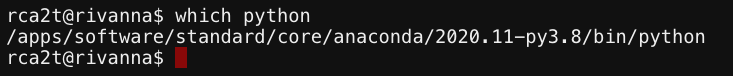
\includegraphics{modules/M02_BasicPython/../../media/which-python.png}

If you do not see ``anaconda'' in that path, then run the following
command:

\begin{Shaded}
\begin{Highlighting}[]
\ExtensionTok{module}\NormalTok{ load anaconda}
\end{Highlighting}
\end{Shaded}

This will update your environment to use Anaconda's distribution of
Python.

After running the command, enter the command to see which pythion is
being used to confirm that it is the one from Ancaconda.

\hypertarget{aside}{%
\section{Aside}\label{aside}}

Note that you can use \texttt{module} to run other programs on your
Rivanna account.

Type \texttt{module\ list} to see which programs have already been
installed on your account.

Type \texttt{module\ spider} to see all the programs you can install.

\hypertarget{the-python-interactive-shell}{%
\section{The Python Interactive
Shell}\label{the-python-interactive-shell}}

From the command line, enter python

You should get the Python Shell:

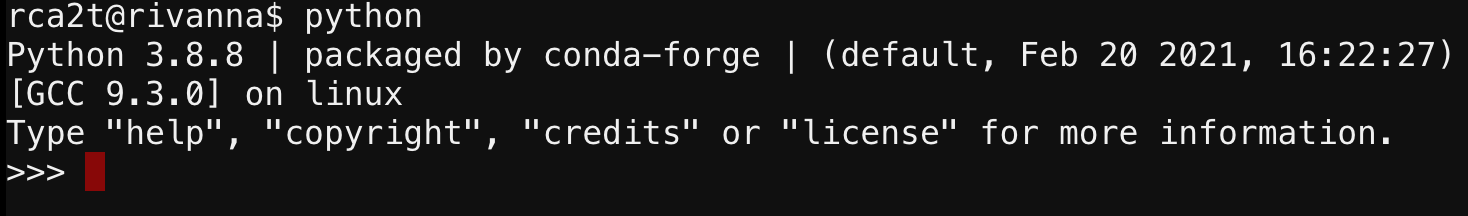
\includegraphics{modules/M02_BasicPython/../../media/python-prompt.png}

This is also called the Python standard REPL, which stands for
``Read-Eval-Print Loop''.

Make sure you see that you are using version 3 of Python.

If you see Python 2, exit the shell by entering \texttt{quit()} and try
again by entering python3 at the command line.

At the \texttt{\textgreater{}\textgreater{}\textgreater{}} prompt type
\texttt{print("Hello,\ World!")} and press return.

If you've never used Python, you've just completed an important ritual.
If you have used Python, well, you did it again :-)

\hypertarget{try-this}{%
\section{\texorpdfstring{Try \texttt{this}}{Try this}}\label{try-this}}

Now, enter following line at the prompt and press return:

\begin{Shaded}
\begin{Highlighting}[]
\ImportTok{import}\NormalTok{ this}
\end{Highlighting}
\end{Shaded}

What do you see?

To exit the Python Shell, enter \texttt{quit()} or \texttt{exit()} and
hit return.

\hypertarget{running-python-files}{%
\section{Running Python Files}\label{running-python-files}}

Now create a file called \texttt{hello.py} using the command line editor
\texttt{nano}. Enter the same commands you used above.

Then run it from the command line by directly invoking the Python
interpreter python.

\begin{tcolorbox}[enhanced jigsaw, toprule=.15mm, opacityback=0, opacitybacktitle=0.6, colback=white, breakable, title=\textcolor{quarto-callout-note-color}{\faInfo}\hspace{0.5em}{Note}, toptitle=1mm, left=2mm, titlerule=0mm, bottomtitle=1mm, rightrule=.15mm, coltitle=black, colbacktitle=quarto-callout-note-color!10!white, colframe=quarto-callout-note-color-frame, arc=.35mm, bottomrule=.15mm, leftrule=.75mm]

See
\href{https://343772-1.kaf.kaltura.com/media/M02\%20Activity\%3A\%20Hello\%2C\%20World!/1_mk92k4i5}{video}
in Canvas.

\end{tcolorbox}

\hypertarget{activity-jupyter-lab}{%
\chapter{Activity: Jupyter Lab}\label{activity-jupyter-lab}}

Now that we have run Python on Rivanna from the command line, let's try
it using a Jupyter Notebook.

Go the OnDemand site to access Rivanna. As a reminder, the URL is
\url{https://rivanna-portal.hpc.virginia.edu/}.

From the Interactive Apps menu, select JupyterLab and fill out the form
to initiate a new session. Your form should have the following values:

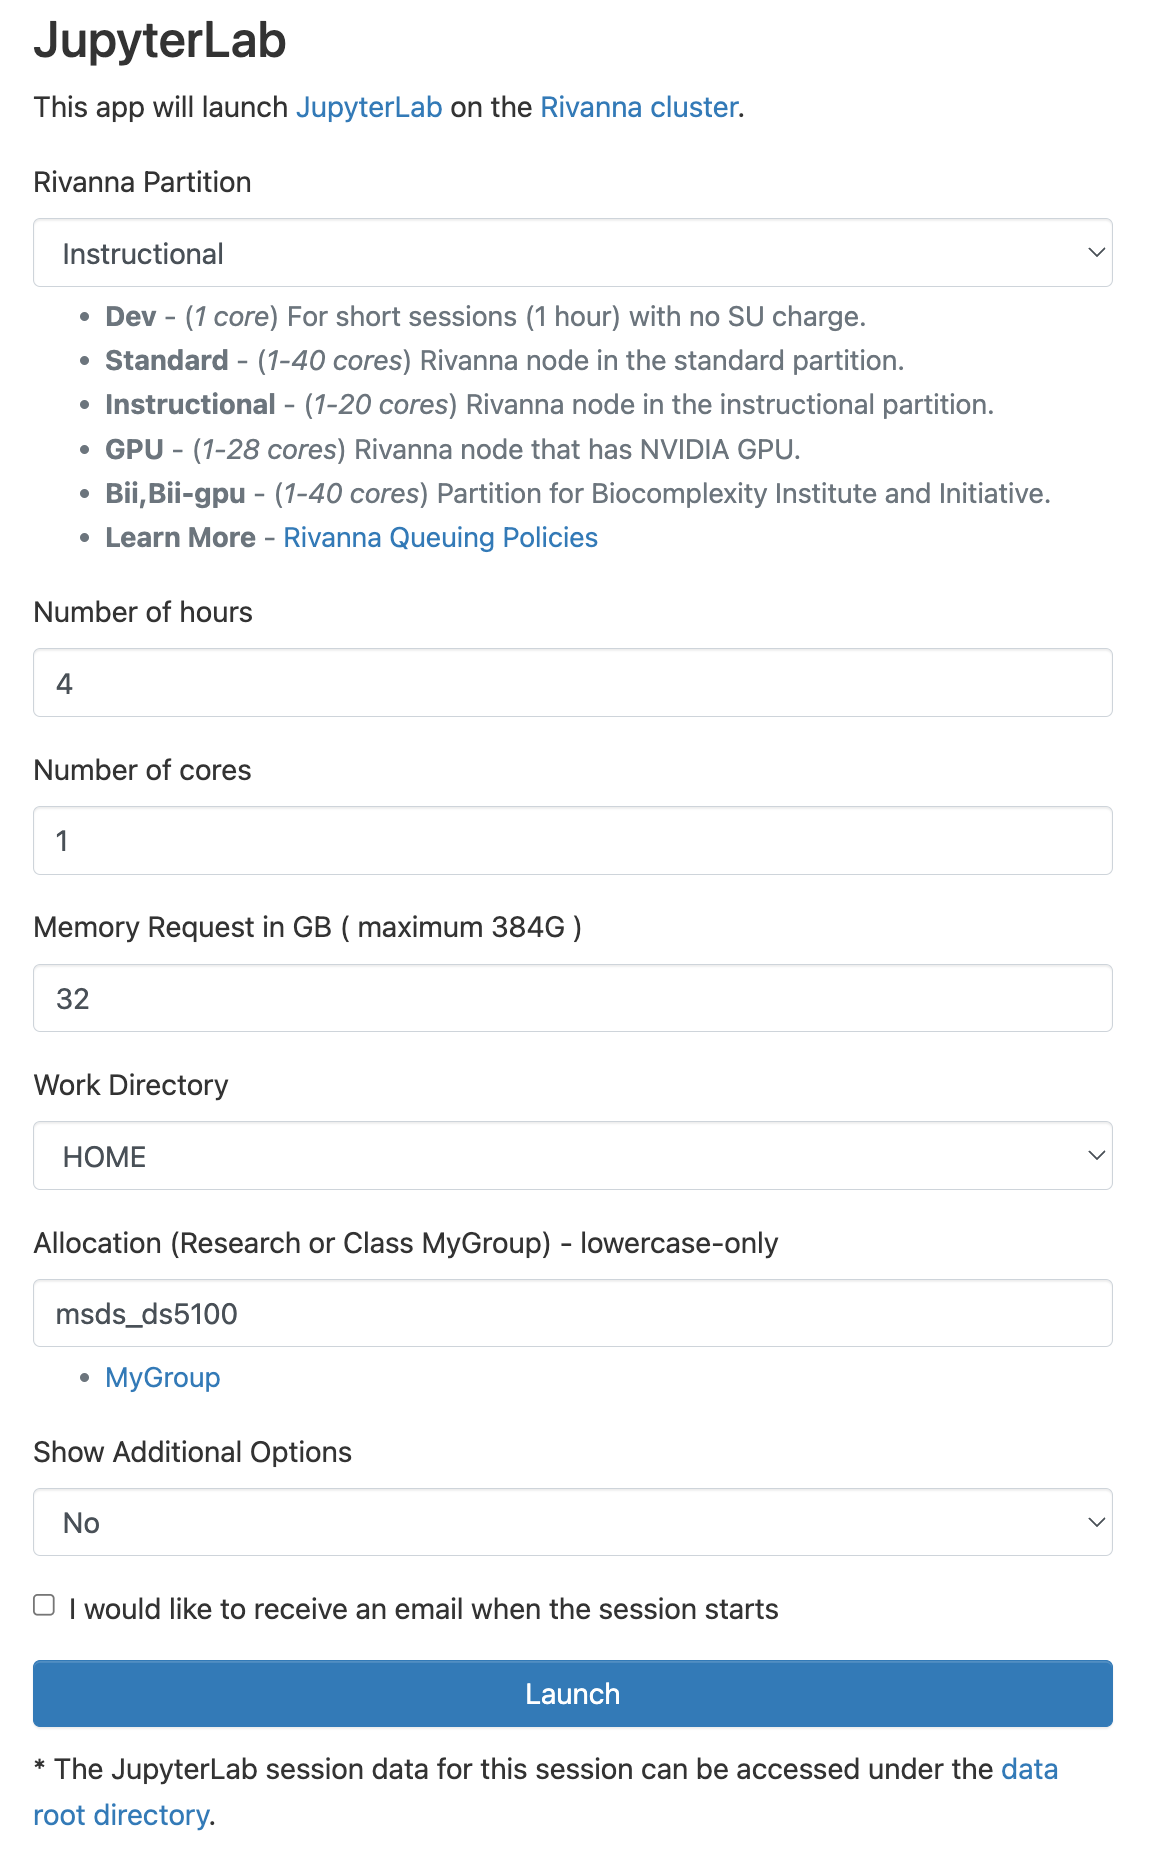
\includegraphics{modules/M02_BasicPython/../../media/jupyter-on-rivanna-form.png}

\begin{tcolorbox}[enhanced jigsaw, toprule=.15mm, opacityback=0, opacitybacktitle=0.6, colback=white, breakable, title=\textcolor{quarto-callout-tip-color}{\faLightbulb}\hspace{0.5em}{Tip}, toptitle=1mm, left=2mm, titlerule=0mm, bottomtitle=1mm, rightrule=.15mm, coltitle=black, colbacktitle=quarto-callout-tip-color!10!white, colframe=quarto-callout-tip-color-frame, arc=.35mm, bottomrule=.15mm, leftrule=.75mm]

Note that you may increase the number of hours, cores, and megabytes of
RAM, but asking for too much will increase the time it takes to start
your session. So select just the resources needed and enter our course
allocation \texttt{?var:course\_allocation} if this value is different
than in the image above).

\end{tcolorbox}

Once the session is ready, launch the notebook.

Once you are in the notebook, use file system tab on the left to get to
the directory of your personal assessments repo. Remember, you created
two repos for this class --- one for course content from the instructor,
and one for your own course work. Use the latter for this exercise.

In a code cell in the notebook, enter the code to print
\texttt{"Hello,\ World!"}, and run the cell.

Save your notebook as \texttt{hello-world.ipynb}.

\hypertarget{nb-data-types-operators-and-expressions}{%
\chapter{NB: Data Types, Operators, and
Expressions}\label{nb-data-types-operators-and-expressions}}

\hypertarget{python-data-types}{%
\chapter{Python Data Types}\label{python-data-types}}

We declare a number of variables with different value types.

By `type' we mean object type.

Data types and data structures are both types of object.

Data types are created by the way they are written or as keywords
\ldots{}

Here is a series of literal values (called \textbf{literals}):

\textbf{Integers}

\begin{Shaded}
\begin{Highlighting}[]
\DecValTok{100}
\end{Highlighting}
\end{Shaded}

\begin{verbatim}
100
\end{verbatim}

\textbf{Floats (decimals)}

\begin{Shaded}
\begin{Highlighting}[]
\FloatTok{3.14} 
\end{Highlighting}
\end{Shaded}

\begin{verbatim}
3.14
\end{verbatim}

\begin{Shaded}
\begin{Highlighting}[]
\DecValTok{1}\NormalTok{, }\FloatTok{1.}
\end{Highlighting}
\end{Shaded}

\begin{verbatim}
(1, 1.0)
\end{verbatim}

\textbf{Strings}

Type of quote does not matter, but they must be straight quotes, not
``smart quotes'' that some word processors use.

Note that there is no explicit \textbf{character} type as in Java and
other languages.

\begin{Shaded}
\begin{Highlighting}[]
\CommentTok{"foo"} 
\end{Highlighting}
\end{Shaded}

\begin{verbatim}
'foo'
\end{verbatim}

\begin{Shaded}
\begin{Highlighting}[]
\CommentTok{"1"}
\end{Highlighting}
\end{Shaded}

\begin{verbatim}
'1'
\end{verbatim}

\begin{Shaded}
\begin{Highlighting}[]
\CommentTok{\textquotesingle{}foo\textquotesingle{}}
\end{Highlighting}
\end{Shaded}

\begin{verbatim}
'foo'
\end{verbatim}

\textbf{Boolean}

\begin{Shaded}
\begin{Highlighting}[]
\VariableTok{True}\NormalTok{, }\VariableTok{False}
\end{Highlighting}
\end{Shaded}

\begin{verbatim}
(True, False)
\end{verbatim}

\textbf{Nothing}

It evaluates to nothing!

\begin{Shaded}
\begin{Highlighting}[]
\VariableTok{None}
\end{Highlighting}
\end{Shaded}

\begin{Shaded}
\begin{Highlighting}[]
\BuiltInTok{print}\NormalTok{(}\VariableTok{None}\NormalTok{)}
\end{Highlighting}
\end{Shaded}

\begin{verbatim}
None
\end{verbatim}

\textbf{Complex}

For the physicists and signal processors.

\begin{Shaded}
\begin{Highlighting}[]
\DecValTok{5}\OperatorTok{+}\OtherTok{0j}
\end{Highlighting}
\end{Shaded}

\begin{verbatim}
(5+0j)
\end{verbatim}

\hypertarget{getting-the-type-of-a-value}{%
\chapter{Getting the type of a
value}\label{getting-the-type-of-a-value}}

You can always find out what kind of type you are working with by
calling the \texttt{type()} function.

\begin{Shaded}
\begin{Highlighting}[]
\BuiltInTok{type}\NormalTok{(}\FloatTok{3.14}\NormalTok{)}
\BuiltInTok{type}\NormalTok{(}\StringTok{"foo"}\NormalTok{)}
\BuiltInTok{type}\NormalTok{(}\StringTok{\textquotesingle{}foo\textquotesingle{}}\NormalTok{)}
\BuiltInTok{type}\NormalTok{(}\VariableTok{True}\NormalTok{)}
\BuiltInTok{type}\NormalTok{(}\VariableTok{None}\NormalTok{)}
\end{Highlighting}
\end{Shaded}

\begin{verbatim}
<class 'float'>
<class 'str'>
<class 'str'>
<class 'bool'>
<class 'NoneType'>
\end{verbatim}

\hypertarget{assignment}{%
\chapter{Assignment}\label{assignment}}

Data are assigned to \textbf{variables} using the assignment
\textbf{operator} \texttt{=}.

The variable is always on the \textbf{left}, the value assigned to it on
the \textbf{right}.

This is not the same as mathemtical equality.

Variables are assigned types \textbf{dynamically}.

This is in contrast to static typing, where you have define variables by
asserting what kind of data values they can hold.

Python figures out what type of data is being set to the variable and
implicitly stores that info.

\begin{Shaded}
\begin{Highlighting}[]
\NormalTok{integerEx }\OperatorTok{=} \DecValTok{8}
\NormalTok{longIntEx }\OperatorTok{=} \DecValTok{22000000000000000000000}
\NormalTok{floatEx }\OperatorTok{=} \FloatTok{2.2}
\NormalTok{stringEx }\OperatorTok{=} \StringTok{"Hello"}
\NormalTok{booleanEx }\OperatorTok{=} \VariableTok{True}
\NormalTok{noneEx }\OperatorTok{=} \VariableTok{None}
\end{Highlighting}
\end{Shaded}

Note that \texttt{type()} returns the type of the value that a variable
holds, not the type ``variable''.

\begin{Shaded}
\begin{Highlighting}[]
\BuiltInTok{type}\NormalTok{(integerEx)}
\end{Highlighting}
\end{Shaded}

\begin{verbatim}
<class 'int'>
\end{verbatim}

\hypertarget{deleting-variables-with-del}{%
\chapter{\texorpdfstring{Deleting variables with
\texttt{del()}}{Deleting variables with del()}}\label{deleting-variables-with-del}}

\begin{Shaded}
\begin{Highlighting}[]
\NormalTok{x }\OperatorTok{=} \FloatTok{101.25}
\end{Highlighting}
\end{Shaded}

\begin{Shaded}
\begin{Highlighting}[]
\NormalTok{x}
\end{Highlighting}
\end{Shaded}

\begin{verbatim}
101.25
\end{verbatim}

\begin{Shaded}
\begin{Highlighting}[]
\KeywordTok{del}\NormalTok{(x)  }\CommentTok{\# delete the variable x}
\end{Highlighting}
\end{Shaded}

\begin{Shaded}
\begin{Highlighting}[]
\NormalTok{x}
\end{Highlighting}
\end{Shaded}

\begin{verbatim}
NameError: name 'x' is not defined
\end{verbatim}

You can't delete values!

\begin{Shaded}
\begin{Highlighting}[]
\KeywordTok{del}\NormalTok{(}\StringTok{"foo"}\NormalTok{)}
\end{Highlighting}
\end{Shaded}

\begin{verbatim}
SyntaxError: cannot delete literal (1397139688.py, line 1)
\end{verbatim}

\hypertarget{get-object-indenity-with-id}{%
\chapter{\texorpdfstring{Get Object Indenity with
\texttt{id()}}{Get Object Indenity with id()}}\label{get-object-indenity-with-id}}

This function returns the identity of an object.

The identity is a number that is guaranteed to be unique and constant
for this object during its lifetime (during the program session).

You can think of it as the address of the object in memory.

\begin{Shaded}
\begin{Highlighting}[]
\BuiltInTok{print}\NormalTok{(}\BuiltInTok{id}\NormalTok{(integerEx))}
\end{Highlighting}
\end{Shaded}

\begin{verbatim}
4329876032
\end{verbatim}

\hypertarget{convert-types-with-casting-functions}{%
\chapter{Convert Types with Casting
Functions}\label{convert-types-with-casting-functions}}

It is possible to convert between types (when it makes sense to do so).

Sometimes conversions are ``lossy'' -- you lose information in the
process

\hypertarget{int}{%
\section{\texorpdfstring{\texttt{int()}}{int()}}\label{int}}

\begin{Shaded}
\begin{Highlighting}[]
\BuiltInTok{int}\NormalTok{?}
\end{Highlighting}
\end{Shaded}

\begin{verbatim}
Init signature: int(self, /, *args, **kwargs)
Docstring:     
int([x]) -> integer
int(x, base=10) -> integer

Convert a number or string to an integer, or return 0 if no arguments
are given.  If x is a number, return x.__int__().  For floating point
numbers, this truncates towards zero.

If x is not a number or if base is given, then x must be a string,
bytes, or bytearray instance representing an integer literal in the
given base.  The literal can be preceded by '+' or '-' and be surrounded
by whitespace.  The base defaults to 10.  Valid bases are 0 and 2-36.
Base 0 means to interpret the base from the string as an integer literal.
>>> int('0b100', base=0)
4
Type:           type
Subclasses:     bool, IntEnum, IntFlag, _NamedIntConstant
\end{verbatim}

\textbf{Float to Int}

\begin{Shaded}
\begin{Highlighting}[]
\NormalTok{val }\OperatorTok{=} \FloatTok{3.8}
\BuiltInTok{print}\NormalTok{(val, }\BuiltInTok{type}\NormalTok{(val))}
\end{Highlighting}
\end{Shaded}

\begin{verbatim}
3.8 <class 'float'>
\end{verbatim}

\begin{Shaded}
\begin{Highlighting}[]
\NormalTok{val\_int }\OperatorTok{=} \BuiltInTok{int}\NormalTok{(val)}
\BuiltInTok{print}\NormalTok{(val\_int, }\BuiltInTok{type}\NormalTok{(val\_int))}
\end{Highlighting}
\end{Shaded}

\begin{verbatim}
3 <class 'int'>
\end{verbatim}

\textbf{String to Float}

\begin{Shaded}
\begin{Highlighting}[]
\NormalTok{val }\OperatorTok{=} \StringTok{\textquotesingle{}3.8\textquotesingle{}}
\BuiltInTok{print}\NormalTok{(val, }\BuiltInTok{type}\NormalTok{(val))}
\end{Highlighting}
\end{Shaded}

\begin{verbatim}
3.8 <class 'str'>
\end{verbatim}

\begin{Shaded}
\begin{Highlighting}[]
\NormalTok{val\_int }\OperatorTok{=} \BuiltInTok{float}\NormalTok{(val)}
\BuiltInTok{print}\NormalTok{(val\_int, }\BuiltInTok{type}\NormalTok{(val\_int))}
\end{Highlighting}
\end{Shaded}

\begin{verbatim}
3.8 <class 'float'>
\end{verbatim}

\textbf{Converting string decimal to integer will fail:}

\begin{Shaded}
\begin{Highlighting}[]
\NormalTok{val }\OperatorTok{=} \StringTok{\textquotesingle{}3.8\textquotesingle{}}
\BuiltInTok{print}\NormalTok{(val, }\BuiltInTok{type}\NormalTok{(val))}
\end{Highlighting}
\end{Shaded}

\begin{verbatim}
3.8 <class 'str'>
\end{verbatim}

\begin{Shaded}
\begin{Highlighting}[]
\NormalTok{val\_int }\OperatorTok{=} \BuiltInTok{int}\NormalTok{(val)}
\BuiltInTok{print}\NormalTok{(val\_int, }\BuiltInTok{type}\NormalTok{(val\_int))}
\end{Highlighting}
\end{Shaded}

\begin{verbatim}
ValueError: invalid literal for int() with base 10: '3.8'
\end{verbatim}

\hypertarget{ord}{%
\section{\texorpdfstring{\texttt{ord()}}{ord()}}\label{ord}}

\textbf{Converting a character to it's code point}

\begin{Shaded}
\begin{Highlighting}[]
\BuiltInTok{ord}\NormalTok{?}
\end{Highlighting}
\end{Shaded}

\begin{verbatim}
Signature: ord(c, /)
Docstring: Return the Unicode code point for a one-character string.
Type:      builtin_function_or_method
\end{verbatim}

\begin{Shaded}
\begin{Highlighting}[]
\BuiltInTok{ord}\NormalTok{(}\StringTok{\textquotesingle{}a\textquotesingle{}}\NormalTok{), }\BuiltInTok{ord}\NormalTok{(}\StringTok{\textquotesingle{}A\textquotesingle{}}\NormalTok{)}
\end{Highlighting}
\end{Shaded}

\begin{verbatim}
(97, 65)
\end{verbatim}

\hypertarget{operators}{%
\chapter{Operators}\label{operators}}

If variables are \textbf{nouns}, and values \textbf{meanings}, then
operators are \textbf{verbs}.

In effect, they are \textbf{elementary functions} that are expressed in
sequential syntax.

\texttt{a\ +\ b} could have been expressed as \texttt{add(a,\ b)}.

Basically, \textbf{each data type is associated with a set of operators}
that allow you to manipulate the data in way that makes sense for its
type. Numeric data types are subject to mathematical operations,
booleans to logical ones, and so forth.

There are also \textbf{operations appropriate to structures}. For
example, list-like things have membership.

The relationship between types and operators is a microcosm of the
relationship betweed data structures and algorithms. \textbf{Data
structures imply algorithms and algorithms assume data structures.}

The w3schools site has
\href{https://www.w3schools.com/python/python_operators.asp}{a good
summary}.

Here are some you may not have seen.

\hypertarget{arithmetic-operators}{%
\section{Arithmetic Operators}\label{arithmetic-operators}}

\hypertarget{floor-division}{%
\subsection{\texorpdfstring{floor division
\texttt{//}}{floor division //}}\label{floor-division}}

\begin{Shaded}
\begin{Highlighting}[]
\DecValTok{5} \OperatorTok{//} \DecValTok{2}
\end{Highlighting}
\end{Shaded}

\begin{verbatim}
2
\end{verbatim}

\begin{Shaded}
\begin{Highlighting}[]
\OperatorTok{{-}}\DecValTok{5} \OperatorTok{//} \DecValTok{2}
\end{Highlighting}
\end{Shaded}

\begin{verbatim}
-3
\end{verbatim}

\begin{Shaded}
\begin{Highlighting}[]
\FloatTok{5.5} \OperatorTok{//} \DecValTok{2}
\end{Highlighting}
\end{Shaded}

\begin{verbatim}
2.0
\end{verbatim}

\hypertarget{modulus}}{modulus \%}}\label{modulus}}

Returns the remainder

\begin{Shaded}
\begin{Highlighting}[]
\DecValTok{5} \OperatorTok{\%} \DecValTok{2}
\end{Highlighting}
\end{Shaded}

\begin{verbatim}
1
\end{verbatim}

odd integers \% 2 = 1\\
even integers \% 2 = 0

Look at this \ldots{}

\begin{Shaded}
\begin{Highlighting}[]
\FloatTok{5.5} \OperatorTok{/} \DecValTok{2}\NormalTok{, }\FloatTok{5.5} \OperatorTok{//} \DecValTok{2}\NormalTok{, }\FloatTok{5.5} \OperatorTok{\%} \DecValTok{2}
\end{Highlighting}
\end{Shaded}

\begin{verbatim}
(2.75, 2.0, 1.5)
\end{verbatim}

\hypertarget{exponentiation}{%
\subsection{\texorpdfstring{exponentiation
\texttt{**}}{exponentiation **}}\label{exponentiation}}

\begin{Shaded}
\begin{Highlighting}[]
\DecValTok{5}\OperatorTok{**}\DecValTok{3}
\end{Highlighting}
\end{Shaded}

\begin{verbatim}
125
\end{verbatim}

\hypertarget{string-operators}{%
\section{String Operators}\label{string-operators}}

\hypertarget{concatenation}{%
\subsection{\texorpdfstring{concatenation
\texttt{+}}{concatenation +}}\label{concatenation}}

The plus sign is an \textbf{ovderloaded} operator in Python.

\begin{Shaded}
\begin{Highlighting}[]
\NormalTok{myString }\OperatorTok{=} \StringTok{\textquotesingle{}This: \textquotesingle{}}
\end{Highlighting}
\end{Shaded}

\begin{Shaded}
\begin{Highlighting}[]
\NormalTok{my2ndString }\OperatorTok{=}\NormalTok{ myString }\OperatorTok{+} \StringTok{\textquotesingle{} Goodbye, world!\textquotesingle{}}
\end{Highlighting}
\end{Shaded}

\begin{Shaded}
\begin{Highlighting}[]
\NormalTok{my2ndString}
\end{Highlighting}
\end{Shaded}

\begin{verbatim}
'This:  Goodbye, world!'
\end{verbatim}

\hypertarget{repetition}{%
\subsection{\texorpdfstring{repetition
\texttt{*}}{repetition *}}\label{repetition}}

\begin{Shaded}
\begin{Highlighting}[]
\CommentTok{\# print(\textquotesingle{}{-}\textquotesingle{} * 80)}
\end{Highlighting}
\end{Shaded}

\begin{Shaded}
\begin{Highlighting}[]
\NormalTok{myString}\OperatorTok{*}\DecValTok{2}                     
\end{Highlighting}
\end{Shaded}

\begin{verbatim}
'This: This: '
\end{verbatim}

\begin{Shaded}
\begin{Highlighting}[]
\NormalTok{myString }\OperatorTok{*} \DecValTok{5}
\end{Highlighting}
\end{Shaded}

\begin{verbatim}
'This: This: This: This: This: '
\end{verbatim}

\begin{Shaded}
\begin{Highlighting}[]
\NormalTok{bart\_S1E3 }\OperatorTok{=} \StringTok{\textquotesingle{}I will not skateboard in the halls\textquotesingle{}}
\end{Highlighting}
\end{Shaded}

\begin{Shaded}
\begin{Highlighting}[]
\BuiltInTok{print}\NormalTok{((bart\_S1E3 }\OperatorTok{+} \StringTok{\textquotesingle{}}\CharTok{\textbackslash{}n}\StringTok{\textquotesingle{}}\NormalTok{) }\OperatorTok{*} \DecValTok{5}\NormalTok{)}
\end{Highlighting}
\end{Shaded}

\begin{verbatim}
I will not skateboard in the halls
I will not skateboard in the halls
I will not skateboard in the halls
I will not skateboard in the halls
I will not skateboard in the halls
\end{verbatim}

\begin{Shaded}
\begin{Highlighting}[]
\BuiltInTok{print}\NormalTok{(}\StringTok{\textquotesingle{}{-}\textquotesingle{}} \OperatorTok{*} \DecValTok{80}\NormalTok{)}
\end{Highlighting}
\end{Shaded}

\begin{verbatim}
--------------------------------------------------------------------------------
\end{verbatim}

\href{https://simpsonswiki.com/wiki/List_of_chalkboard_gags}{See them
all} :-)

\hypertarget{assignment-operator}{%
\section{\texorpdfstring{Assignment Operator
\texttt{=}}{Assignment Operator =}}\label{assignment-operator}}

We've used this already, but it too is an operator.

\begin{Shaded}
\begin{Highlighting}[]
\NormalTok{epoch }\OperatorTok{=} \DecValTok{20}
\BuiltInTok{print}\NormalTok{(}\StringTok{\textquotesingle{}epoch:\textquotesingle{}}\NormalTok{, epoch)}
\end{Highlighting}
\end{Shaded}

\begin{verbatim}
epoch: 20
\end{verbatim}

\hypertarget{comparison-operators}{%
\section{Comparison Operators}\label{comparison-operators}}

Comparisons are questions.

They return a boolean value.

\hypertarget{equality} \DecValTok{5}\NormalTok{)}
\end{Highlighting}
\end{Shaded}

\begin{verbatim}
True
\end{verbatim}

\begin{Shaded}
\begin{Highlighting}[]
\CommentTok{\textquotesingle{}Boo\textquotesingle{}} \OperatorTok{==} \StringTok{\textquotesingle{}Hoo\textquotesingle{}}
\end{Highlighting}
\end{Shaded}

\begin{verbatim}
False
\end{verbatim}

Can we compare strings

\begin{Shaded}
\begin{Highlighting}[]
\CommentTok{\textquotesingle{}A\textquotesingle{}} \OperatorTok{\textless{}} \StringTok{\textquotesingle{}B\textquotesingle{}}
\end{Highlighting}
\end{Shaded}

\begin{verbatim}
True
\end{verbatim}

\begin{Shaded}
\begin{Highlighting}[]
\BuiltInTok{ord}\NormalTok{(}\StringTok{\textquotesingle{}A\textquotesingle{}}\NormalTok{), }\BuiltInTok{ord}\NormalTok{(}\StringTok{\textquotesingle{}B\textquotesingle{}}\NormalTok{)}
\end{Highlighting}
\end{Shaded}

\begin{verbatim}
(65, 66)
\end{verbatim}

\hypertarget{inequality}{%
\subsection{\texorpdfstring{inequality
\texttt{!=}}{inequality !=}}\label{inequality}}

\begin{Shaded}
\begin{Highlighting}[]
\DecValTok{5}\OperatorTok{/}\DecValTok{9} \OperatorTok{!=} \FloatTok{0.5555}
\end{Highlighting}
\end{Shaded}

\begin{verbatim}
True
\end{verbatim}

\hypertarget{logical-operators}{%
\section{Logical Operators}\label{logical-operators}}

Python uses words where other languages will use other symbols.

\hypertarget{conjunctions-and-or-not} \DecValTok{10} \OperatorTok{==} \DecValTok{0}\NormalTok{) }\KeywordTok{or}\NormalTok{ (x }\OperatorTok{\textless{}} \OperatorTok{{-}}\DecValTok{1}\NormalTok{)}
\end{Highlighting}
\end{Shaded}

\begin{verbatim}
True
\end{verbatim}

\begin{Shaded}
\begin{Highlighting}[]
\NormalTok{(x }\OperatorTok{\%} \DecValTok{10} \OperatorTok{==} \DecValTok{0}\NormalTok{) }\KeywordTok{and}\NormalTok{ (x }\OperatorTok{\textless{}} \OperatorTok{{-}}\DecValTok{1}\NormalTok{)}
\end{Highlighting}
\end{Shaded}

\begin{verbatim}
False
\end{verbatim}

\begin{Shaded}
\begin{Highlighting}[]
\KeywordTok{not}\NormalTok{ x }\OperatorTok{==} \DecValTok{5}
\end{Highlighting}
\end{Shaded}

\begin{verbatim}
True
\end{verbatim}

\hypertarget{identity-is}{%
\subsection{\texorpdfstring{Identity
\texttt{is}}{Identity is}}\label{identity-is}}

The \texttt{is} keyword is used to test if two variables refer to the
same object.

The test returns \texttt{True} if the two objects are the same object.

The test returns False if they are not the same object, even if the two
objects are 100\% equal.

Use the \texttt{==} operator to test if two variables are equal.

-- from
\href{https://www.w3schools.com/python/gloss_python_identity_operators.asp}{W3Schools
on Identity Operators}

\texttt{is}

\begin{Shaded}
\begin{Highlighting}[]
\NormalTok{x }\OperatorTok{=} \StringTok{\textquotesingle{}fail\textquotesingle{}}
\end{Highlighting}
\end{Shaded}

\begin{Shaded}
\begin{Highlighting}[]
\NormalTok{x }\KeywordTok{is} \StringTok{\textquotesingle{}fail\textquotesingle{}}
\end{Highlighting}
\end{Shaded}

\begin{verbatim}
<>:1: SyntaxWarning: "is" with a literal. Did you mean "=="?
<>:1: SyntaxWarning: "is" with a literal. Did you mean "=="?
/var/folders/14/rnyfspnx2q131jp_752t9fc80000gn/T/ipykernel_53814/1139635342.py:1: SyntaxWarning: "is" with a literal. Did you mean "=="?
  x is 'fail'
\end{verbatim}

\begin{verbatim}
True
\end{verbatim}

\texttt{is\ not}

\begin{Shaded}
\begin{Highlighting}[]
\NormalTok{x }\KeywordTok{is} \KeywordTok{not} \StringTok{\textquotesingle{}fail\textquotesingle{}}
\end{Highlighting}
\end{Shaded}

\begin{verbatim}
<>:1: SyntaxWarning: "is not" with a literal. Did you mean "!="?
<>:1: SyntaxWarning: "is not" with a literal. Did you mean "!="?
/var/folders/14/rnyfspnx2q131jp_752t9fc80000gn/T/ipykernel_53814/1754352910.py:1: SyntaxWarning: "is not" with a literal. Did you mean "!="?
  x is not 'fail'
\end{verbatim}

\begin{verbatim}
False
\end{verbatim}

\begin{Shaded}
\begin{Highlighting}[]
\NormalTok{x }\OperatorTok{=} \StringTok{\textquotesingle{}foo\textquotesingle{}}
\NormalTok{y }\OperatorTok{=} \StringTok{\textquotesingle{}foo\textquotesingle{}}
\NormalTok{x }\KeywordTok{is}\NormalTok{ y}
\end{Highlighting}
\end{Shaded}

\begin{verbatim}
True
\end{verbatim}

\begin{Shaded}
\begin{Highlighting}[]
\NormalTok{x }\OperatorTok{=}\NormalTok{ [}\StringTok{\textquotesingle{}a\textquotesingle{}}\NormalTok{]}
\NormalTok{y }\OperatorTok{=}\NormalTok{ [}\StringTok{\textquotesingle{}a\textquotesingle{}}\NormalTok{]}
\NormalTok{x }\KeywordTok{is}\NormalTok{ y}
\end{Highlighting}
\end{Shaded}

\begin{verbatim}
False
\end{verbatim}

\hypertarget{negation-not}{%
\subsection{\texorpdfstring{Negation
\texttt{not}}{Negation not}}\label{negation-not}}

\begin{Shaded}
\begin{Highlighting}[]
\KeywordTok{not} \VariableTok{True}\NormalTok{, }\KeywordTok{not} \VariableTok{False}\NormalTok{, }\KeywordTok{not} \DecValTok{0}\NormalTok{, }\KeywordTok{not} \DecValTok{1}\NormalTok{, }\KeywordTok{not} \DecValTok{1000}\NormalTok{, }\KeywordTok{not} \VariableTok{None}
\end{Highlighting}
\end{Shaded}

\begin{verbatim}
(False, True, True, False, False, True)
\end{verbatim}

\hypertarget{unary-operators}{%
\chapter{Unary Operators}\label{unary-operators}}

Python offers a short-cut for most operators. When updating a variable
with an operation to that variable, such as:

\begin{Shaded}
\begin{Highlighting}[]
\NormalTok{my\_var }\OperatorTok{=}\NormalTok{ my\_var }\OperatorTok{+} \DecValTok{1}  \CommentTok{\# Incrementing}
\end{Highlighting}
\end{Shaded}

You can do this:

\begin{Shaded}
\begin{Highlighting}[]
\NormalTok{my\_var }\OperatorTok{+=} \DecValTok{1}
\end{Highlighting}
\end{Shaded}

Python supports many operators this way. Here are some:

\begin{Shaded}
\begin{Highlighting}[]
\NormalTok{a }\OperatorTok{{-}=}\NormalTok{ a}
\NormalTok{a \textbackslash{}}\OperatorTok{=}\NormalTok{ a}
\NormalTok{a \textbackslash{}\textbackslash{}}\OperatorTok{=}\NormalTok{ a}
\NormalTok{a }\OperatorTok{\%=}\NormalTok{ a}
\NormalTok{a }\OperatorTok{*=}\NormalTok{ a}
\NormalTok{a }\OperatorTok{**=}\NormalTok{ a}
\end{Highlighting}
\end{Shaded}

\hypertarget{expressions}{%
\chapter{Expressions}\label{expressions}}

Variables, literal values, and operators are the building blocks of
ebxpressions.

For example, the following combines three operators and four variables:

\begin{Shaded}
\begin{Highlighting}[]
\DecValTok{1} \OperatorTok{+} \DecValTok{2} \OperatorTok{*} \DecValTok{3} \OperatorTok{/} \DecValTok{2}
\end{Highlighting}
\end{Shaded}

\begin{verbatim}
4.0
\end{verbatim}

Python employs \textbf{operator precedence} when evaluating expressions:

\begin{verbatim}
P – Parentheses
E – Exponentiation
M – Multiplication
D – Division
A – Addition
S – Subtraction
\end{verbatim}

You can use parentheses to group them to force the order of operations
you want:

\begin{Shaded}
\begin{Highlighting}[]
\NormalTok{(}\DecValTok{1} \OperatorTok{+} \DecValTok{2}\NormalTok{) }\OperatorTok{*}\NormalTok{ (}\DecValTok{3} \OperatorTok{/} \DecValTok{2}\NormalTok{)}
\end{Highlighting}
\end{Shaded}

\begin{verbatim}
4.5
\end{verbatim}

Variables and literal values can be combined:

\begin{Shaded}
\begin{Highlighting}[]
\NormalTok{y }\OperatorTok{=} \DecValTok{5}
\NormalTok{m }\OperatorTok{=} \FloatTok{2.5}
\NormalTok{b }\OperatorTok{=} \DecValTok{10}
\end{Highlighting}
\end{Shaded}

\begin{Shaded}
\begin{Highlighting}[]
\NormalTok{y }\OperatorTok{=}\NormalTok{ m }\OperatorTok{*} \DecValTok{10} \OperatorTok{+}\NormalTok{ b}
\NormalTok{y}
\end{Highlighting}
\end{Shaded}

\begin{verbatim}
35.0
\end{verbatim}

\begin{Shaded}
\begin{Highlighting}[]
\NormalTok{y }\OperatorTok{=}\NormalTok{ m }\OperatorTok{*} \DecValTok{5} \OperatorTok{+}\NormalTok{ b}
\NormalTok{y}
\end{Highlighting}
\end{Shaded}

\begin{verbatim}
22.5
\end{verbatim}

Expresssion can be very complex.

Expressions evaluate to a value, just as single variables do.

Therefore, they can be put anywhere a value is accepted.

\begin{Shaded}
\begin{Highlighting}[]
\BuiltInTok{int}\NormalTok{((y }\OperatorTok{+} \DecValTok{10}\NormalTok{) }\OperatorTok{**} \DecValTok{8}\NormalTok{)}
\end{Highlighting}
\end{Shaded}

\begin{verbatim}
1244706300354
\end{verbatim}

\hypertarget{nb-numbers}{%
\chapter{NB: Numbers}\label{nb-numbers}}

These are built-in mathematical functions for numbers.

\hypertarget{pow-power}{%
\section{\texorpdfstring{\texttt{pow()}
Power}{pow() Power}}\label{pow-power}}

\begin{Shaded}
\begin{Highlighting}[]
\BuiltInTok{pow}\NormalTok{(}\DecValTok{2}\NormalTok{,}\DecValTok{3}\NormalTok{) }\CommentTok{\# 2 raised to 3 = 8}
\end{Highlighting}
\end{Shaded}

\hypertarget{abs-absolute-value}{%
\section{\texorpdfstring{\texttt{abs()} Absolute
value}{abs() Absolute value}}\label{abs-absolute-value}}

\begin{Shaded}
\begin{Highlighting}[]
\BuiltInTok{abs}\NormalTok{(}\OperatorTok{{-}}\DecValTok{2}\NormalTok{) }\CommentTok{\# returns 2, the absolute value of its argument}
\end{Highlighting}
\end{Shaded}

\hypertarget{round-round}{%
\section{\texorpdfstring{\texttt{round()}
Round}{round() Round}}\label{round-round}}

Rounding up or down its argument (to closest whole number).

\begin{Shaded}
\begin{Highlighting}[]
\BuiltInTok{round}\NormalTok{(}\FloatTok{2.8}\NormalTok{) }\CommentTok{\# rounds up to 3.0}
\end{Highlighting}
\end{Shaded}

\begin{verbatim}
3
\end{verbatim}

\begin{Shaded}
\begin{Highlighting}[]
\BuiltInTok{round}\NormalTok{(}\FloatTok{1.1}\NormalTok{) }\CommentTok{\# rounds down to 1.0}
\end{Highlighting}
\end{Shaded}

\begin{verbatim}
1
\end{verbatim}

\hypertarget{math-library-functions}{%
\chapter{Math library functions}\label{math-library-functions}}

See the Python docs on
\href{https://docs.python.org/3/library/math.html}{the math library}.

\begin{Shaded}
\begin{Highlighting}[]
\ImportTok{import}\NormalTok{ math}
\end{Highlighting}
\end{Shaded}

\hypertarget{math.sqrt-square-root}{%
\section{\texorpdfstring{\texttt{math.sqrt()} Square
root}{math.sqrt() Square root}}\label{math.sqrt-square-root}}

\begin{Shaded}
\begin{Highlighting}[]
\NormalTok{math.sqrt?}
\end{Highlighting}
\end{Shaded}

\begin{verbatim}
Signature: math.sqrt(x, /)
Docstring: Return the square root of x.
Type:      builtin_function_or_method
\end{verbatim}

\begin{Shaded}
\begin{Highlighting}[]
\CommentTok{\# sqrt(intOne)}
\end{Highlighting}
\end{Shaded}

\begin{Shaded}
\begin{Highlighting}[]
\NormalTok{math.sqrt(}\DecValTok{12}\NormalTok{) }\CommentTok{\# using the square{-}root function from the math library}
\end{Highlighting}
\end{Shaded}

\begin{verbatim}
3.4641016151377544
\end{verbatim}

\begin{Shaded}
\begin{Highlighting}[]
\BuiltInTok{print}\NormalTok{(math.floor(}\FloatTok{2.5}\NormalTok{)) }\CommentTok{\# returns largest whole number less than the argument}
\BuiltInTok{print}\NormalTok{(math.floor(}\FloatTok{2.9}\NormalTok{))}
\BuiltInTok{print}\NormalTok{(math.floor(}\FloatTok{2.1}\NormalTok{))}
\end{Highlighting}
\end{Shaded}

\begin{verbatim}
2
2
2
\end{verbatim}

\hypertarget{math.log}{%
\section{\texorpdfstring{\texttt{math.log()}}{math.log()}}\label{math.log}}

\begin{Shaded}
\begin{Highlighting}[]
\NormalTok{math.log?}
\end{Highlighting}
\end{Shaded}

\begin{Shaded}
\begin{Highlighting}[]
\NormalTok{math.log(}\DecValTok{100}\NormalTok{, }\DecValTok{10}\NormalTok{)}
\end{Highlighting}
\end{Shaded}

\begin{Shaded}
\begin{Highlighting}[]
\NormalTok{math.log(}\DecValTok{256}\NormalTok{, }\DecValTok{2}\NormalTok{)}
\end{Highlighting}
\end{Shaded}

\hypertarget{the-random-library}{%
\chapter{The Random library}\label{the-random-library}}

See \href{https://docs.python.org/3/library/random.html}{random ---
Generate pseudo-random numbers} for more info.

\begin{Shaded}
\begin{Highlighting}[]
\ImportTok{import}\NormalTok{ random}
\end{Highlighting}
\end{Shaded}

\hypertarget{random.random}{%
\section{\texorpdfstring{\texttt{random.random()}}{random.random()}}\label{random.random}}

\begin{Shaded}
\begin{Highlighting}[]
\NormalTok{random.random?}
\end{Highlighting}
\end{Shaded}

\begin{Shaded}
\begin{Highlighting}[]
\BuiltInTok{print}\NormalTok{(random.random()) }\CommentTok{\# using random() function in random library}
    \CommentTok{\# will return a number between 0 and 1}
\end{Highlighting}
\end{Shaded}

\hypertarget{random.randint}{%
\section{\texorpdfstring{\texttt{random.randint()}}{random.randint()}}\label{random.randint}}

\begin{Shaded}
\begin{Highlighting}[]
\NormalTok{random.randint?}
\end{Highlighting}
\end{Shaded}

\begin{Shaded}
\begin{Highlighting}[]
\BuiltInTok{print}\NormalTok{(random.randint(}\DecValTok{1}\NormalTok{,}\DecValTok{100}\NormalTok{)) }\CommentTok{\# specify a range in the parenthesis}
    \CommentTok{\# this will return a random integer in the range 1{-}100}
\end{Highlighting}
\end{Shaded}

\hypertarget{nb-booleans}{%
\chapter{NB: Booleans}\label{nb-booleans}}

A \texttt{boolean} value takes one of \texttt{True} or \texttt{False},
which are built-in values

check if \texttt{cache} is True, using \texttt{if} statement\\
\texttt{if} statement using a bool evaluates to True or False

\begin{Shaded}
\begin{Highlighting}[]
\NormalTok{cache }\OperatorTok{=} \VariableTok{True}

\ControlFlowTok{if}\NormalTok{ cache:}
   \BuiltInTok{print}\NormalTok{(}\StringTok{\textquotesingle{}data will be cached\textquotesingle{}}\NormalTok{)}
\end{Highlighting}
\end{Shaded}

\begin{verbatim}
data will be cached
\end{verbatim}

\begin{Shaded}
\begin{Highlighting}[]
\BuiltInTok{print}\NormalTok{(}\BuiltInTok{type}\NormalTok{(cache))}
\end{Highlighting}
\end{Shaded}

\begin{verbatim}
<class 'bool'>
\end{verbatim}

\textbf{Booleans are frequently used in \texttt{if/then} statements.}

We'll cover these later.

\begin{Shaded}
\begin{Highlighting}[]
\NormalTok{cache }\OperatorTok{=} \VariableTok{True}
\NormalTok{oome }\OperatorTok{=} \VariableTok{False}

\ControlFlowTok{if}\NormalTok{ cache }\KeywordTok{or}\NormalTok{ oome:}
    \BuiltInTok{print}\NormalTok{(}\StringTok{\textquotesingle{}condition met!\textquotesingle{}}\NormalTok{)}
\ControlFlowTok{else}\NormalTok{:}
    \BuiltInTok{print}\NormalTok{(}\StringTok{"No dice."}\NormalTok{)}
\end{Highlighting}
\end{Shaded}

AND statements will short circuit if an early condition fails.

\begin{Shaded}
\begin{Highlighting}[]
\ControlFlowTok{if}\NormalTok{ oome }\KeywordTok{and}\NormalTok{ cache:}
    \BuiltInTok{print}\NormalTok{(}\StringTok{\textquotesingle{}condition met!\textquotesingle{}}\NormalTok{)}
\end{Highlighting}
\end{Shaded}

In this case, since \emph{oome} is False, the check on \emph{cache}
never happens.

\hypertarget{nb-strings}{%
\chapter{NB: Strings}\label{nb-strings}}

Strings are signified by quotes.

Single and double quotes are identical in function.

They must be ``straight quotes'' though -- cutting and pasting from a
Word document with smart quotes won't work.

\begin{Shaded}
\begin{Highlighting}[]
\CommentTok{\textquotesingle{}hello world!\textquotesingle{}} \OperatorTok{==} \StringTok{"hello world!"}
\end{Highlighting}
\end{Shaded}

\hypertarget{quote-prefixes}{%
\section{Quote prefixes}\label{quote-prefixes}}

\hypertarget{r-strings}{%
\subsection{\texorpdfstring{\texttt{r}
strings}{r strings}}\label{r-strings}}

Prefixing a string causes escape characters to be uninterpreted.

\begin{Shaded}
\begin{Highlighting}[]
\BuiltInTok{print}\NormalTok{(}\StringTok{"Sentence one.}\CharTok{\textbackslash{}n}\StringTok{Sentence two."}\NormalTok{)}
\end{Highlighting}
\end{Shaded}

\begin{Shaded}
\begin{Highlighting}[]
\BuiltInTok{print}\NormalTok{(}\VerbatimStringTok{r"Sentence one.\textbackslash{}nSentence two."}\NormalTok{)}
\end{Highlighting}
\end{Shaded}

\hypertarget{f-strings}{%
\subsection{\texorpdfstring{\texttt{f}
strings}{f strings}}\label{f-strings}}

Prefixing a string with \texttt{f} allows variable interpolation --
inplace evaluation of variables in strings.

\begin{Shaded}
\begin{Highlighting}[]
\NormalTok{ppl }\OperatorTok{=} \StringTok{\textquotesingle{}knights\textquotesingle{}}
\NormalTok{greeting }\OperatorTok{=} \StringTok{\textquotesingle{}Ni\textquotesingle{}}
\end{Highlighting}
\end{Shaded}

\begin{Shaded}
\begin{Highlighting}[]
\BuiltInTok{print}\NormalTok{(}\SpecialStringTok{f\textquotesingle{}We are the }\SpecialCharTok{\{}\NormalTok{ppl}\SpecialCharTok{\}}\SpecialStringTok{ who say }\SpecialCharTok{\{}\NormalTok{greeting}\SpecialCharTok{\}}\SpecialStringTok{!\textquotesingle{}}\NormalTok{) }\CommentTok{\# Output: We are the knights who say Ni!}
\end{Highlighting}
\end{Shaded}

The brackets and characters within them (called format fields) are
replaced with the passed objects.

\begin{Shaded}
\begin{Highlighting}[]
\BuiltInTok{print}\NormalTok{(}\StringTok{b"This is a sentence."}\NormalTok{)}
\end{Highlighting}
\end{Shaded}

\begin{Shaded}
\begin{Highlighting}[]
\BuiltInTok{print}\NormalTok{(}\StringTok{"This is a sentence."}\NormalTok{)}
\end{Highlighting}
\end{Shaded}

\hypertarget{printing-print}{%
\chapter{\texorpdfstring{Printing
\texttt{print()}}{Printing print()}}\label{printing-print}}

Python uses a print function.

\begin{Shaded}
\begin{Highlighting}[]
\BuiltInTok{print}\NormalTok{(}\StringTok{"This is a simple print statement"}\NormalTok{)}
\end{Highlighting}
\end{Shaded}

Python supports special ``escape characters'' in strings that produce
effects when printed.

\begin{verbatim}
\\     Backslash (\)
\'     Single quote (')
\"     Double quote (")
\n     ASCII Linefeed, aka new line
\end{verbatim}

Note that these are not unique to Python. They are part of almost all
languages.

\begin{Shaded}
\begin{Highlighting}[]
\CommentTok{\# Tab character ( \textbackslash{}t )}
\BuiltInTok{print}\NormalTok{(}\StringTok{"Hello,}\CharTok{\textbackslash{}t}\StringTok{World! (With a tab character)"}\NormalTok{)}
\end{Highlighting}
\end{Shaded}

\begin{verbatim}
Hello,  World! (With a tab character)
\end{verbatim}

\begin{Shaded}
\begin{Highlighting}[]
\CommentTok{\# Inserting a new line (line feed) character ( \textbackslash{}n )}
\BuiltInTok{print}\NormalTok{(}\StringTok{"Line one}\CharTok{\textbackslash{}n}\StringTok{Line two, with newline character"}\NormalTok{)}
\end{Highlighting}
\end{Shaded}

\begin{verbatim}
Line one
Line two, with newline character
\end{verbatim}

\begin{Shaded}
\begin{Highlighting}[]
\CommentTok{\# Concatenation in strings: }
\CommentTok{\# Use plus sign ( + ) to concatenate the parts of the string}
\BuiltInTok{print}\NormalTok{(}\StringTok{"Concatenation,"} \OperatorTok{+} \StringTok{"}\CharTok{\textbackslash{}t}\StringTok{"} \OperatorTok{+} \StringTok{"in strings with tab in middle"}\NormalTok{)}
\end{Highlighting}
\end{Shaded}

\begin{Shaded}
\begin{Highlighting}[]
\CommentTok{\# If you wanted to print special characters}
\CommentTok{\# Printing quotes}
\BuiltInTok{print}\NormalTok{(}\StringTok{\textquotesingle{}Printing "quotes" within a string\textquotesingle{}}\NormalTok{) }\CommentTok{\# mixing single and double quotes}
\end{Highlighting}
\end{Shaded}

\begin{Shaded}
\begin{Highlighting}[]
\CommentTok{\# What if you needed to print special characters like (\textbackslash{}) or (\textquotesingle{}) or (")}
\BuiltInTok{print}\NormalTok{(}\StringTok{\textquotesingle{}If I want to print }\CharTok{\textbackslash{}\textquotesingle{}}\StringTok{single quotes}\CharTok{\textbackslash{}\textquotesingle{}}\StringTok{ in a string, use backslash!\textquotesingle{}}\NormalTok{)}
\BuiltInTok{print}\NormalTok{(}\StringTok{"If I want to print }\CharTok{\textbackslash{}"}\StringTok{double quotes}\CharTok{\textbackslash{}"}\StringTok{ in a string, use backslash!"}\NormalTok{)}
\BuiltInTok{print}\NormalTok{(}\StringTok{\textquotesingle{}If I want to print }\CharTok{\textbackslash{}\textbackslash{}}\StringTok{the backslash}\CharTok{\textbackslash{}\textbackslash{}}\StringTok{ in a string, also use backslash!\textquotesingle{}}\NormalTok{)}
\end{Highlighting}
\end{Shaded}

\begin{verbatim}
If I want to print 'single quotes' in a string, use backslash!
If I want to print "double quotes" in a string, use backslash!
If I want to print \the backslash\ in a string, also use backslash!
\end{verbatim}

The print function puts spaces between strings and a newline at the end,
but you can change that:

\begin{Shaded}
\begin{Highlighting}[]
\BuiltInTok{print}\NormalTok{(}\StringTok{"This"}\NormalTok{, }\StringTok{"is"}\NormalTok{, }\StringTok{"a"}\NormalTok{, }\StringTok{"sentence"}\NormalTok{)}
\end{Highlighting}
\end{Shaded}

\begin{Shaded}
\begin{Highlighting}[]
\BuiltInTok{print}\NormalTok{(}\StringTok{"This"}\NormalTok{, }\StringTok{"is"}\NormalTok{, }\StringTok{"a"}\NormalTok{, }\StringTok{"sentence"}\NormalTok{, sep}\OperatorTok{=}\StringTok{"{-}{-}"}\NormalTok{)}
\end{Highlighting}
\end{Shaded}

\begin{Shaded}
\begin{Highlighting}[]
\BuiltInTok{print}\NormalTok{(}\StringTok{"This"}\NormalTok{, }\StringTok{"is"}\NormalTok{, }\StringTok{"a"}\NormalTok{, }\StringTok{"sentence"}\NormalTok{)}
\BuiltInTok{print}\NormalTok{(}\StringTok{"This"}\NormalTok{, }\StringTok{"is"}\NormalTok{, }\StringTok{"a"}\NormalTok{, }\StringTok{"sentence"}\NormalTok{)}
\end{Highlighting}
\end{Shaded}

\begin{Shaded}
\begin{Highlighting}[]
\BuiltInTok{print}\NormalTok{(}\StringTok{"This"}\NormalTok{, }\StringTok{"is"}\NormalTok{, }\StringTok{"a"}\NormalTok{, }\StringTok{"sentence"}\NormalTok{, end}\OperatorTok{=}\StringTok{" | "}\NormalTok{)}
\BuiltInTok{print}\NormalTok{(}\StringTok{"This"}\NormalTok{, }\StringTok{"is"}\NormalTok{, }\StringTok{"a"}\NormalTok{, }\StringTok{"sentence"}\NormalTok{)}
\end{Highlighting}
\end{Shaded}

\hypertarget{comments}{%
\chapter{Comments}\label{comments}}

Comments are lines of code that aren't read by the interpreter.

They are used to explain blocks of code, or to remove code from
execution when debugging.

\begin{Shaded}
\begin{Highlighting}[]
\CommentTok{\# This is single{-}line comment}
\end{Highlighting}
\end{Shaded}

These following are multiline strings that can serve as comments:

\begin{Shaded}
\begin{Highlighting}[]
\NormalTok{foo }\OperatorTok{=} \StringTok{\textquotesingle{}\textquotesingle{}\textquotesingle{}}
\StringTok{This is an}
\StringTok{example of}
\StringTok{a multi{-}line}
\StringTok{comment: single quotes}
\StringTok{\textquotesingle{}\textquotesingle{}\textquotesingle{}}
\end{Highlighting}
\end{Shaded}

\begin{Shaded}
\begin{Highlighting}[]
\NormalTok{foo}
\end{Highlighting}
\end{Shaded}

\begin{verbatim}
'\nThis is an\nexample of\na multi-line\ncomment: single quotes\n'
\end{verbatim}

\begin{Shaded}
\begin{Highlighting}[]
\BuiltInTok{print}\NormalTok{(foo)}
\end{Highlighting}
\end{Shaded}

\begin{verbatim}

This is an
example of
a multi-line
comment: single quotes
\end{verbatim}

\begin{Shaded}
\begin{Highlighting}[]
\CommentTok{"""}
\CommentTok{Here is another}
\CommentTok{example of}
\CommentTok{a multi{-}line}
\CommentTok{comment: double quotes}
\CommentTok{"""}
\end{Highlighting}
\end{Shaded}

Note that multiline comments also evaluate as values.

\hypertarget{run-time-user-input}{%
\chapter{Run-time User Input}\label{run-time-user-input}}

\begin{Shaded}
\begin{Highlighting}[]
\NormalTok{answer }\OperatorTok{=} \BuiltInTok{input}\NormalTok{(}\StringTok{"What is your name? "}\NormalTok{)}
\BuiltInTok{print}\NormalTok{(}\StringTok{"Hello, "} \OperatorTok{+}\NormalTok{ answer }\OperatorTok{+} \StringTok{"!"}\NormalTok{)}
\end{Highlighting}
\end{Shaded}

\hypertarget{some-string-functions}{%
\chapter{Some String Functions}\label{some-string-functions}}

\begin{Shaded}
\begin{Highlighting}[]
\NormalTok{Built}\OperatorTok{{-}}\KeywordTok{in}\NormalTok{ string methods }\KeywordTok{and}\NormalTok{ functions.}

\NormalTok{See [Common String Operations](https:}\OperatorTok{//}\NormalTok{docs.python.org}\OperatorTok{/}\DecValTok{3}\OperatorTok{/}\NormalTok{library}\OperatorTok{/}\NormalTok{string.html) }\ControlFlowTok{for}\NormalTok{ more info.}
\end{Highlighting}
\end{Shaded}

\hypertarget{lower-.upper}{%
\section{\texorpdfstring{\texttt{.lower()},
\texttt{.upper()}}{.lower(), .upper()}}\label{lower-.upper}}

\begin{Shaded}
\begin{Highlighting}[]
\CommentTok{\textquotesingle{}BOB\textquotesingle{}}\NormalTok{.lower() }\CommentTok{\#.upper()}
\end{Highlighting}
\end{Shaded}

\begin{verbatim}
'bob'
\end{verbatim}

\hypertarget{split}{%
\section{\texorpdfstring{\texttt{.split()}}{.split()}}\label{split}}

Parase a string based on a delimiter, which defaults to whitespace.

NOTE: This does \emph{not} use regular expressions.

This returns a list.

\begin{Shaded}
\begin{Highlighting}[]
\NormalTok{montyPythonQuote }\OperatorTok{=} \StringTok{\textquotesingle{}are.you.suggesting.coconuts.migrate\textquotesingle{}}
\end{Highlighting}
\end{Shaded}

\begin{Shaded}
\begin{Highlighting}[]
\CommentTok{\textquotesingle{}are.you.suggesting.coconuts.migrate\textquotesingle{}}\NormalTok{.split(}\StringTok{\textquotesingle{}.\textquotesingle{}}\NormalTok{)}
\end{Highlighting}
\end{Shaded}

\begin{verbatim}
['are', 'you', 'suggesting', 'coconuts', 'migrate']
\end{verbatim}

\begin{Shaded}
\begin{Highlighting}[]
\NormalTok{montyPythonQuote}
\end{Highlighting}
\end{Shaded}

\begin{verbatim}
'are.you.suggesting.coconuts.migrate'
\end{verbatim}

\begin{Shaded}
\begin{Highlighting}[]
\NormalTok{montyPythonQuote.split(}\StringTok{\textquotesingle{}.\textquotesingle{}}\NormalTok{) }\CommentTok{\# split by the \textquotesingle{}.\textquotesingle{} delimiter. Result: a list!}
\end{Highlighting}
\end{Shaded}

\begin{verbatim}
['are', 'you', 'suggesting', 'coconuts', 'migrate']
\end{verbatim}

\hypertarget{strip-.rstrip-lstrip-strip-methods}{%
\section{\texorpdfstring{\texttt{.strip()}, \texttt{.rstrip()},
\texttt{lstrip()} Strip
methods}{.strip(), .rstrip(), lstrip() Strip methods}}\label{strip-.rstrip-lstrip-strip-methods}}

Strip out extra whitespace using strip(), rstrip() and lstrip()
functions

\texttt{.strip()} removes white space from anywhere\\
\texttt{.rstrip()} only removes white space from the right-hand-side of
the string\\
\texttt{.lstrip()} only removes white space from the left-hand-side of
the string

\begin{Shaded}
\begin{Highlighting}[]
\NormalTok{str1 }\OperatorTok{=} \StringTok{\textquotesingle{}  hello, world!\textquotesingle{}}    \CommentTok{\# white space at the beginning}
\NormalTok{str2 }\OperatorTok{=} \StringTok{\textquotesingle{}  hello, world!  \textquotesingle{}}  \CommentTok{\# white space at both ends}
\NormalTok{str3 }\OperatorTok{=} \StringTok{\textquotesingle{}hello, world!  \textquotesingle{}}    \CommentTok{\# white space at the end}
\end{Highlighting}
\end{Shaded}

\begin{Shaded}
\begin{Highlighting}[]
\NormalTok{str1, str2, str3}
\end{Highlighting}
\end{Shaded}

\begin{Shaded}
\begin{Highlighting}[]
\NormalTok{str1.lstrip(), str1.rstrip()}
\end{Highlighting}
\end{Shaded}

\begin{Shaded}
\begin{Highlighting}[]
\NormalTok{str2.strip(), str2.rstrip()}
\end{Highlighting}
\end{Shaded}

\begin{Shaded}
\begin{Highlighting}[]
\NormalTok{str2.lstrip(), str3.rstrip()}
\end{Highlighting}
\end{Shaded}

\begin{Shaded}
\begin{Highlighting}[]
\NormalTok{status.startswith(}\StringTok{\textquotesingle{}a\textquotesingle{}}\NormalTok{)}
\end{Highlighting}
\end{Shaded}

\begin{Shaded}
\begin{Highlighting}[]
\NormalTok{status.endswith(}\StringTok{\textquotesingle{}s\textquotesingle{}}\NormalTok{)}
\end{Highlighting}
\end{Shaded}

\hypertarget{replace}{%
\section{\texorpdfstring{\texttt{.replace()}}{.replace()}}\label{replace}}

\begin{Shaded}
\begin{Highlighting}[]
\CommentTok{"latina"}\NormalTok{.replace(}\StringTok{"a"}\NormalTok{, }\StringTok{"x"}\NormalTok{)}
\end{Highlighting}
\end{Shaded}

\hypertarget{format}{%
\section{\texorpdfstring{\texttt{.format()}}{.format()}}\label{format}}

Variable values can be embedding in strings using the \texttt{format()}
function.\\
Place \{\} in the string in order from left to right. followed by
\texttt{.format(var1,\ var2,\ ...})`

\begin{Shaded}
\begin{Highlighting}[]
\NormalTok{epoch }\OperatorTok{=} \DecValTok{20}
\NormalTok{loss }\OperatorTok{=} \FloatTok{1.55}

\BuiltInTok{print}\NormalTok{(}\StringTok{\textquotesingle{}Epoch: }\SpecialCharTok{\{\}}\StringTok{, loss: }\SpecialCharTok{\{\}}\StringTok{\textquotesingle{}}\NormalTok{.}\BuiltInTok{format}\NormalTok{(epoch, loss))}
\end{Highlighting}
\end{Shaded}

This breaks, as three variables are required based on number of \{\}

\begin{Shaded}
\begin{Highlighting}[]
\BuiltInTok{print}\NormalTok{(}\StringTok{\textquotesingle{}Epoch: }\SpecialCharTok{\{\}}\StringTok{, loop: }\SpecialCharTok{\{\}}\StringTok{, loss: }\SpecialCharTok{\{\}}\StringTok{\textquotesingle{}}\NormalTok{.}\BuiltInTok{format}\NormalTok{(epoch, loss))}
\end{Highlighting}
\end{Shaded}

\hypertarget{zfill}{%
\section{\texorpdfstring{\texttt{.zfill()}}{.zfill()}}\label{zfill}}

Basic usage of the str.zfill() method (pads a numeric string on the left
with zeros) It understands about plus and minus signs

\begin{Shaded}
\begin{Highlighting}[]
\BuiltInTok{print}\NormalTok{(}\StringTok{\textquotesingle{}12\textquotesingle{}}\NormalTok{.zfill(}\DecValTok{5}\NormalTok{))       }\CommentTok{\# Output: 00012}
\BuiltInTok{print}\NormalTok{(}\StringTok{\textquotesingle{}{-}3.14\textquotesingle{}}\NormalTok{.zfill(}\DecValTok{7}\NormalTok{))    }\CommentTok{\# Output: {-}003.14}
\BuiltInTok{print}\NormalTok{(}\StringTok{\textquotesingle{}3.141592\textquotesingle{}}\NormalTok{.zfill(}\DecValTok{5}\NormalTok{)) }\CommentTok{\# Output: 3.141592}
\end{Highlighting}
\end{Shaded}

\hypertarget{strings-are-lists}{%
\chapter{Strings are Lists}\label{strings-are-lists}}

Actually, they are list-like.

Here are some functions applicable to strings because they are lists.

\hypertarget{len-length}{%
\section{\texorpdfstring{\texttt{len()}
Length}{len() Length}}\label{len-length}}

This is built-in length funciton tells us how many characters in the
string.

It also applys to any list-like object, including strings, lists, dicts,
sets, and dataframes.

\begin{Shaded}
\begin{Highlighting}[]
\BuiltInTok{len}\NormalTok{?}
\end{Highlighting}
\end{Shaded}

\begin{Shaded}
\begin{Highlighting}[]
\NormalTok{my\_new\_tring }\OperatorTok{=} \StringTok{\textquotesingle{}This is a string\textquotesingle{}}
\end{Highlighting}
\end{Shaded}

\begin{Shaded}
\begin{Highlighting}[]
\BuiltInTok{len}\NormalTok{(my\_new\_tring)}
\end{Highlighting}
\end{Shaded}

\hypertarget{indexing}{%
\subsection{Indexing}\label{indexing}}

Since strings are sequences in Python, each character of the string has
a unique position that can be indexed.

Indexes are indicated by suffixed brackets, e.g.~\texttt{foo{[}{]}}

\begin{Shaded}
\begin{Highlighting}[]
\NormalTok{my\_new\_tring[}\DecValTok{0}\NormalTok{] }\CommentTok{\# displays the first character of the string}
            \CommentTok{\# first position is position zero. Will display \textquotesingle{}h\textquotesingle{}}
\end{Highlighting}
\end{Shaded}

\begin{Shaded}
\begin{Highlighting}[]
\NormalTok{my\_new\_tring[}\OperatorTok{{-}}\DecValTok{1}\NormalTok{] }\CommentTok{\# displays the last character. Negatives count backwords.}
\end{Highlighting}
\end{Shaded}

\hypertarget{slicing}{%
\subsection{Slicing}\label{slicing}}

We can used the colon to `slice' strings (and lists)

\begin{Shaded}
\begin{Highlighting}[]
\NormalTok{my\_new\_tring[}\DecValTok{0}\NormalTok{:}\DecValTok{4}\NormalTok{] }\CommentTok{\# First four characters (index positions 0{-}3)}
\end{Highlighting}
\end{Shaded}

\begin{Shaded}
\begin{Highlighting}[]
\NormalTok{my\_new\_tring[:}\DecValTok{4}\NormalTok{]  }\CommentTok{\# Beginning (0) to (n{-}1) position}
\end{Highlighting}
\end{Shaded}

\begin{Shaded}
\begin{Highlighting}[]
\NormalTok{my\_new\_tring[}\DecValTok{4}\NormalTok{:]  }\CommentTok{\# Fifth character and onwards until the end of the string}
\end{Highlighting}
\end{Shaded}

it is NOT possible to reassign elements of a string. Python strings are
\textbf{immutable}.

\begin{Shaded}
\begin{Highlighting}[]
\NormalTok{status }\OperatorTok{=} \StringTok{\textquotesingle{}success\textquotesingle{}}
\NormalTok{status[}\DecValTok{0}\NormalTok{] }\OperatorTok{=} \StringTok{\textquotesingle{}t\textquotesingle{}}
\end{Highlighting}
\end{Shaded}

Add strings and handle pathing

\hypertarget{nb-structures}{%
\chapter{NB: Structures}\label{nb-structures}}

In contrast to primitive data types, data structures organize types into
structures that have certain properties, such as \textbf{order},
\textbf{mutability}, and \textbf{addressing scheme}, e.g.~by index.

A list is an ordered sequence of items.

Each element of a list is associated with an integer that represents the
order in which the element appears.

Lists are indexed with \textbf{brackets} \texttt{{[}{]}}.

List elements are accessed by providing their order number in the
brackets.

Lists are \textbf{mutable}, meaning you can modify them after they have
been created.

They can contain mixed types.

\hypertarget{constructing}{%
\section{Constructing}\label{constructing}}

They can be \textbf{constructed} in several ways:

\begin{Shaded}
\begin{Highlighting}[]
\NormalTok{list1 }\OperatorTok{=}\NormalTok{ []}
\NormalTok{list2 }\OperatorTok{=} \BuiltInTok{list}\NormalTok{()}
\NormalTok{list3 }\OperatorTok{=} \StringTok{"some string"}\NormalTok{.split()}
\NormalTok{numbers }\OperatorTok{=}\NormalTok{ [}\DecValTok{1}\NormalTok{,}\DecValTok{2}\NormalTok{,}\DecValTok{3}\NormalTok{,}\DecValTok{4}\NormalTok{] }
\end{Highlighting}
\end{Shaded}

\hypertarget{indexing-1}{%
\section{Indexing}\label{indexing-1}}

\textbf{Zero-based indexing}

Python uses xzero-based indexing, which means for a collection
\texttt{mylist}

\texttt{mylist{[}0{]}} references the first element\\
\texttt{mylist{[}1{]}} references the second element, etc

For any iterable object of length \emph{N}:\\
\texttt{mylist{[}:n{]}} will return the first \emph{n} elements from
index \emph{0} to \emph{n-1}\\
\texttt{mylist{[}-n:{]}} will return the last \emph{n} elements from
index \emph{N-n} to \emph{N-1}

\begin{Shaded}
\begin{Highlighting}[]
\NormalTok{numbers[}\DecValTok{0}\NormalTok{] }\CommentTok{\# Access first element (output: 1)}
\end{Highlighting}
\end{Shaded}

\begin{verbatim}
1
\end{verbatim}

\begin{Shaded}
\begin{Highlighting}[]
\NormalTok{numbers[}\OperatorTok{{-}}\DecValTok{1}\NormalTok{]}
\end{Highlighting}
\end{Shaded}

\begin{verbatim}
4
\end{verbatim}

\begin{Shaded}
\begin{Highlighting}[]
\NormalTok{numbers[}\DecValTok{0}\NormalTok{] }\OperatorTok{+}\NormalTok{ numbers[}\DecValTok{3}\NormalTok{] }\CommentTok{\# doing arithmetic with the values (output: 5)}
\end{Highlighting}
\end{Shaded}

\begin{verbatim}
5
\end{verbatim}

\begin{Shaded}
\begin{Highlighting}[]
\NormalTok{numbers[}\BuiltInTok{len}\NormalTok{(numbers)]}
\end{Highlighting}
\end{Shaded}

\begin{verbatim}
IndexError: list index out of range
\end{verbatim}

\hypertarget{slicing-1}{%
\section{Slicing}\label{slicing-1}}

\begin{Shaded}
\begin{Highlighting}[]
\NormalTok{numbers[}\DecValTok{0}\NormalTok{:}\DecValTok{2}\NormalTok{] }\CommentTok{\# Output: [1, 2]}
\end{Highlighting}
\end{Shaded}

\begin{verbatim}
[1, 2]
\end{verbatim}

\begin{Shaded}
\begin{Highlighting}[]
\NormalTok{numbers[}\DecValTok{1}\NormalTok{:}\DecValTok{3}\NormalTok{] }\CommentTok{\# Output: [2, 3]}
\end{Highlighting}
\end{Shaded}

\begin{verbatim}
[2, 3]
\end{verbatim}

\begin{Shaded}
\begin{Highlighting}[]
\BuiltInTok{len}\NormalTok{(numbers) }\CommentTok{\# use len() function to find the size. Output: 4}
\end{Highlighting}
\end{Shaded}

\begin{verbatim}
4
\end{verbatim}

\begin{Shaded}
\begin{Highlighting}[]
\NormalTok{numbers[}\DecValTok{2}\NormalTok{:]  }\CommentTok{\# Output: [3, 4]}
\end{Highlighting}
\end{Shaded}

\begin{verbatim}
[3, 4]
\end{verbatim}

\hypertarget{multiply-lists-by-a-scalar}{%
\section{Multiply lists by a scalar}\label{multiply-lists-by-a-scalar}}

A scalar is a single value number.

\begin{Shaded}
\begin{Highlighting}[]
\NormalTok{numbers }\OperatorTok{*} \DecValTok{2}
\end{Highlighting}
\end{Shaded}

\hypertarget{concatenate-lists-with}{%
\section{\texorpdfstring{Concatenate lists with
\texttt{+}}{Concatenate lists with +}}\label{concatenate-lists-with}}

\begin{Shaded}
\begin{Highlighting}[]
\NormalTok{numbers2 }\OperatorTok{=}\NormalTok{ [}\DecValTok{30}\NormalTok{, }\DecValTok{40}\NormalTok{, }\DecValTok{50}\NormalTok{]}
\end{Highlighting}
\end{Shaded}

\begin{Shaded}
\begin{Highlighting}[]
\NormalTok{numbers }\OperatorTok{+}\NormalTok{ numbers2 }\CommentTok{\# concatenate two lists}
\end{Highlighting}
\end{Shaded}

\hypertarget{lists-can-mix-types}{%
\section{Lists can mix types}\label{lists-can-mix-types}}

\begin{Shaded}
\begin{Highlighting}[]
\NormalTok{myList }\OperatorTok{=}\NormalTok{ [}\StringTok{\textquotesingle{}coconuts\textquotesingle{}}\NormalTok{, }\DecValTok{777}\NormalTok{, }\FloatTok{7.25}\NormalTok{, }\StringTok{\textquotesingle{}Sir Robin\textquotesingle{}}\NormalTok{, }\FloatTok{80.0}\NormalTok{, }\VariableTok{True}\NormalTok{]}
\end{Highlighting}
\end{Shaded}

\begin{Shaded}
\begin{Highlighting}[]
\NormalTok{myList}
\end{Highlighting}
\end{Shaded}

\textbf{What happens if we multiply a list with strings?}

\begin{Shaded}
\begin{Highlighting}[]
\CommentTok{\# myList * 2}
\end{Highlighting}
\end{Shaded}

\hypertarget{lists-can-be-nested}{%
\section{Lists can be nested}\label{lists-can-be-nested}}

\begin{Shaded}
\begin{Highlighting}[]
\NormalTok{names }\OperatorTok{=}\NormalTok{ [}\StringTok{\textquotesingle{}Darrell\textquotesingle{}}\NormalTok{, }\StringTok{\textquotesingle{}Clayton\textquotesingle{}}\NormalTok{, [}\StringTok{\textquotesingle{}Billie\textquotesingle{}}\NormalTok{, }\StringTok{\textquotesingle{}Arthur\textquotesingle{}}\NormalTok{], }\StringTok{\textquotesingle{}Samantha\textquotesingle{}}\NormalTok{]}
\NormalTok{names[}\DecValTok{2}\NormalTok{] }\CommentTok{\# returns a *list*}
\NormalTok{names[}\DecValTok{0}\NormalTok{] }\CommentTok{\# returns a *string*}
\end{Highlighting}
\end{Shaded}

cannot subset into a float, will break

\begin{Shaded}
\begin{Highlighting}[]
\NormalTok{names[}\DecValTok{2}\NormalTok{][}\DecValTok{0}\NormalTok{]}
\end{Highlighting}
\end{Shaded}

\hypertarget{lists-can-concatenated-with}{%
\section{\texorpdfstring{Lists can concatenated with
\texttt{+}}{Lists can concatenated with +}}\label{lists-can-concatenated-with}}

\begin{Shaded}
\begin{Highlighting}[]
\NormalTok{variables }\OperatorTok{=}\NormalTok{ [}\StringTok{\textquotesingle{}x1\textquotesingle{}}\NormalTok{, }\StringTok{\textquotesingle{}x2\textquotesingle{}}\NormalTok{, }\StringTok{\textquotesingle{}x3\textquotesingle{}}\NormalTok{]}
\NormalTok{response }\OperatorTok{=}\NormalTok{ [}\StringTok{\textquotesingle{}y\textquotesingle{}}\NormalTok{]}
\end{Highlighting}
\end{Shaded}

\begin{Shaded}
\begin{Highlighting}[]
\NormalTok{variables }\OperatorTok{+}\NormalTok{ response}
\end{Highlighting}
\end{Shaded}

\begin{verbatim}
['x1', 'x2', 'x3', 'y']
\end{verbatim}

\hypertarget{dictionaries-dict}{%
\chapter{\texorpdfstring{Dictionaries
\texttt{dict}}{Dictionaries dict}}\label{dictionaries-dict}}

Like a hash table.

Has key-value pairs.

Elements are indexed using brackets \texttt{{[}{]}} (like lists).

But they are constructed used braces \texttt{\{\}}.

Key names are unique. If you re-use a key, you overwrite its value.

Keys don't have to be strings -- they can be numbers or tuples or
expressions that evaluate to one of these.

\hypertarget{constructing-1}{%
\section{Constructing}\label{constructing-1}}

\begin{Shaded}
\begin{Highlighting}[]
\NormalTok{dict1 }\OperatorTok{=}\NormalTok{ \{}
    \StringTok{\textquotesingle{}a\textquotesingle{}}\NormalTok{: }\DecValTok{1}\NormalTok{,}
    \StringTok{\textquotesingle{}b\textquotesingle{}}\NormalTok{: }\DecValTok{2}\NormalTok{,}
    \StringTok{\textquotesingle{}c\textquotesingle{}}\NormalTok{: }\DecValTok{3}
\NormalTok{\}}
\end{Highlighting}
\end{Shaded}

\begin{Shaded}
\begin{Highlighting}[]
\NormalTok{dict2 }\OperatorTok{=} \BuiltInTok{dict}\NormalTok{(x}\OperatorTok{=}\DecValTok{55}\NormalTok{, y}\OperatorTok{=}\DecValTok{29}\NormalTok{, z}\OperatorTok{=}\DecValTok{99}\NormalTok{) }\CommentTok{\# Note the absence of quotes around keys}
\end{Highlighting}
\end{Shaded}

\begin{Shaded}
\begin{Highlighting}[]
\NormalTok{dict2}
\end{Highlighting}
\end{Shaded}

\begin{verbatim}
{'x': 55, 'y': 29, 'z': 99}
\end{verbatim}

\begin{Shaded}
\begin{Highlighting}[]
\NormalTok{dict3 }\OperatorTok{=}\NormalTok{ \{}\StringTok{\textquotesingle{}A\textquotesingle{}}\NormalTok{: }\StringTok{\textquotesingle{}foo\textquotesingle{}}\NormalTok{, }\DecValTok{99}\NormalTok{: }\StringTok{\textquotesingle{}bar\textquotesingle{}}\NormalTok{, (}\DecValTok{1}\NormalTok{,}\DecValTok{2}\NormalTok{): }\StringTok{\textquotesingle{}baz\textquotesingle{}}\NormalTok{\}}
\end{Highlighting}
\end{Shaded}

\begin{Shaded}
\begin{Highlighting}[]
\NormalTok{dict3}
\end{Highlighting}
\end{Shaded}

\begin{verbatim}
{'A': 'foo', 99: 'bar', (1, 2): 'baz'}
\end{verbatim}

\hypertarget{retrieve-a-value}{%
\section{Retrieve a value}\label{retrieve-a-value}}

Just write a key as the \emph{index}.

\begin{Shaded}
\begin{Highlighting}[]
\NormalTok{phonelist }\OperatorTok{=}\NormalTok{ \{}\StringTok{\textquotesingle{}Tom\textquotesingle{}}\NormalTok{:}\DecValTok{123}\NormalTok{, }\StringTok{\textquotesingle{}Bob\textquotesingle{}}\NormalTok{:}\DecValTok{456}\NormalTok{, }\StringTok{\textquotesingle{}Sam\textquotesingle{}}\NormalTok{:}\DecValTok{897}\NormalTok{\}}
\end{Highlighting}
\end{Shaded}

\begin{Shaded}
\begin{Highlighting}[]
\NormalTok{phonelist[}\StringTok{\textquotesingle{}Bob\textquotesingle{}}\NormalTok{]}
\end{Highlighting}
\end{Shaded}

\hypertarget{print-list-of-keys-values-or-both}{%
\section{Print list of keys, values, or
both}\label{print-list-of-keys-values-or-both}}

Use the \texttt{.keys()},
\texttt{.values()\textquotesingle{},\ or}.items()` methods.

Keys are not sorted. For example, they are not ordered in order in which
they were added.

\begin{Shaded}
\begin{Highlighting}[]
\NormalTok{phonelist.keys() }\CommentTok{\# Returns a list}
\end{Highlighting}
\end{Shaded}

\begin{Shaded}
\begin{Highlighting}[]
\NormalTok{phonelist.values() }\CommentTok{\# Returns a list}
\end{Highlighting}
\end{Shaded}

\begin{Shaded}
\begin{Highlighting}[]
\NormalTok{phonelist.items() }\CommentTok{\# Returns a list of tuples}
\end{Highlighting}
\end{Shaded}

\begin{Shaded}
\begin{Highlighting}[]
\NormalTok{phonelist }\CommentTok{\# note the data returned is not the same as the data entered}
\end{Highlighting}
\end{Shaded}

\hypertarget{tuples}{%
\chapter{Tuples}\label{tuples}}

A tuple is like a list but with one big difference: \textbf{a tuple is
an immutable object!}

You can't change a tuple once it's created.

A tuple can contain any number of elements of any datatype.

Accessed with brackets \texttt{{[}{]}} but constructed with parentheses
\texttt{()}.

\begin{Shaded}
\begin{Highlighting}[]
\NormalTok{numbers}
\end{Highlighting}
\end{Shaded}

\hypertarget{constructing-2}{%
\section{Constructing}\label{constructing-2}}

Created with comma-separated values, with or without parenthesis.

\begin{Shaded}
\begin{Highlighting}[]
\NormalTok{letters }\OperatorTok{=} \StringTok{\textquotesingle{}a\textquotesingle{}}\NormalTok{, }\StringTok{\textquotesingle{}b\textquotesingle{}}\NormalTok{, }\StringTok{\textquotesingle{}c\textquotesingle{}}\NormalTok{, }\StringTok{\textquotesingle{}d\textquotesingle{}}
\end{Highlighting}
\end{Shaded}

\begin{Shaded}
\begin{Highlighting}[]
\NormalTok{letters}
\end{Highlighting}
\end{Shaded}

\begin{Shaded}
\begin{Highlighting}[]
\NormalTok{numbers }\OperatorTok{=}\NormalTok{ (}\DecValTok{1}\NormalTok{,}\DecValTok{2}\NormalTok{,}\DecValTok{3}\NormalTok{,}\DecValTok{4}\NormalTok{) }\CommentTok{\# numbers 1,2,3,4 stored in a tuple}
\end{Highlighting}
\end{Shaded}

A single valued tuple must include a comma \texttt{,}, e.g.

\begin{Shaded}
\begin{Highlighting}[]
\NormalTok{tuple0 }\OperatorTok{=}\NormalTok{ (}\DecValTok{29}\NormalTok{)}
\end{Highlighting}
\end{Shaded}

\begin{Shaded}
\begin{Highlighting}[]
\NormalTok{tuple0, }\BuiltInTok{type}\NormalTok{(tuple0)}
\end{Highlighting}
\end{Shaded}

\begin{Shaded}
\begin{Highlighting}[]
\NormalTok{tuple1 }\OperatorTok{=}\NormalTok{ (}\DecValTok{29}\NormalTok{,)}
\end{Highlighting}
\end{Shaded}

\begin{Shaded}
\begin{Highlighting}[]
\NormalTok{tuple1, }\BuiltInTok{type}\NormalTok{(tuple1)}
\end{Highlighting}
\end{Shaded}

\begin{Shaded}
\begin{Highlighting}[]
\BuiltInTok{len}\NormalTok{(numbers)}
\end{Highlighting}
\end{Shaded}

\begin{Shaded}
\begin{Highlighting}[]
\NormalTok{numbers[}\DecValTok{0}\NormalTok{] }\OperatorTok{=} \DecValTok{5} \CommentTok{\# Trying to assign a new value 5 to the first position}
\end{Highlighting}
\end{Shaded}

\hypertarget{common-functions-and-methods-to-all-sequences}{%
\chapter{Common functions and methods to all
sequences}\label{common-functions-and-methods-to-all-sequences}}

\begin{verbatim}
len()
in
+ 
*
\end{verbatim}

\begin{Shaded}
\begin{Highlighting}[]
\NormalTok{[}\DecValTok{1}\NormalTok{, }\DecValTok{3}\NormalTok{] }\OperatorTok{*} \DecValTok{8}
\end{Highlighting}
\end{Shaded}

\begin{Shaded}
\begin{Highlighting}[]
\NormalTok{(}\DecValTok{1}\NormalTok{, }\DecValTok{3}\NormalTok{) }\OperatorTok{*} \DecValTok{8}
\end{Highlighting}
\end{Shaded}

\hypertarget{membership-with-in}{%
\section{\texorpdfstring{Membership with
\texttt{in}}{Membership with in}}\label{membership-with-in}}

Returns a boolean.

\begin{Shaded}
\begin{Highlighting}[]
\CommentTok{\textquotesingle{}Sam\textquotesingle{}} \KeywordTok{in}\NormalTok{ phonelist}
\end{Highlighting}
\end{Shaded}

\hypertarget{sets}{%
\chapter{Sets}\label{sets}}

A \texttt{set} is an unordered collection of unique objects.

They are subject to set operations.

\begin{Shaded}
\begin{Highlighting}[]
\NormalTok{peanuts }\OperatorTok{=}\NormalTok{ \{}\StringTok{\textquotesingle{}snoopy\textquotesingle{}}\NormalTok{,}\StringTok{\textquotesingle{}snoopy\textquotesingle{}}\NormalTok{,}\StringTok{\textquotesingle{}woodstock\textquotesingle{}}\NormalTok{\}}
\end{Highlighting}
\end{Shaded}

\begin{Shaded}
\begin{Highlighting}[]
\NormalTok{peanuts}
\end{Highlighting}
\end{Shaded}

Note the set is deduped

Since sets are unordered, they don't have an index. This will break:

\begin{Shaded}
\begin{Highlighting}[]
\NormalTok{peanuts[}\DecValTok{0}\NormalTok{]}
\end{Highlighting}
\end{Shaded}

\begin{Shaded}
\begin{Highlighting}[]
\ControlFlowTok{for}\NormalTok{ peanut }\KeywordTok{in}\NormalTok{ peanuts:}
    \BuiltInTok{print}\NormalTok{(peanut)}
\end{Highlighting}
\end{Shaded}

\textbf{Check if a value is in the set using \texttt{in}}

\begin{Shaded}
\begin{Highlighting}[]
\CommentTok{\textquotesingle{}snoopy\textquotesingle{}} \KeywordTok{in}\NormalTok{ peanuts}
\end{Highlighting}
\end{Shaded}

Combine two sets

\begin{Shaded}
\begin{Highlighting}[]
\NormalTok{set1 }\OperatorTok{=}\NormalTok{ \{}\StringTok{\textquotesingle{}python\textquotesingle{}}\NormalTok{,}\StringTok{\textquotesingle{}R\textquotesingle{}}\NormalTok{\}}
\NormalTok{set2 }\OperatorTok{=}\NormalTok{ \{}\StringTok{\textquotesingle{}R\textquotesingle{}}\NormalTok{,}\StringTok{\textquotesingle{}SQL\textquotesingle{}}\NormalTok{\}}
\end{Highlighting}
\end{Shaded}

This fails:

\begin{Shaded}
\begin{Highlighting}[]
\NormalTok{set1 }\OperatorTok{+}\NormalTok{ set2}
\end{Highlighting}
\end{Shaded}

This succeeds:

\begin{Shaded}
\begin{Highlighting}[]
\NormalTok{set1.union(set2)}
\end{Highlighting}
\end{Shaded}

Get the set intersection

\begin{Shaded}
\begin{Highlighting}[]
\NormalTok{set1.intersection(set2)}
\end{Highlighting}
\end{Shaded}

\hypertarget{ranges}{%
\chapter{Ranges}\label{ranges}}

A range is a sequence of integers, from \texttt{start} to \texttt{stop}
by \texttt{step}. - The \texttt{start} point is zero by default.\\
- The \texttt{step} is one by default.\\
- The \texttt{stop} point is NOT included.

Ranges can be assigned to a variable.

\begin{Shaded}
\begin{Highlighting}[]
\NormalTok{rng }\OperatorTok{=} \BuiltInTok{range}\NormalTok{(}\DecValTok{5}\NormalTok{)}
\end{Highlighting}
\end{Shaded}

More often, ranges are used in iterations, which we will cover later.

\begin{Shaded}
\begin{Highlighting}[]
\ControlFlowTok{for}\NormalTok{ rn }\KeywordTok{in}\NormalTok{ rng:}
    \BuiltInTok{print}\NormalTok{(rn)}
\end{Highlighting}
\end{Shaded}

another range:

\begin{Shaded}
\begin{Highlighting}[]
\NormalTok{rangy }\OperatorTok{=} \BuiltInTok{range}\NormalTok{(}\DecValTok{1}\NormalTok{, }\DecValTok{11}\NormalTok{, }\DecValTok{2}\NormalTok{)}
\ControlFlowTok{for}\NormalTok{ rn }\KeywordTok{in}\NormalTok{ rangy:}
    \BuiltInTok{print}\NormalTok{(rn)}
\end{Highlighting}
\end{Shaded}

\hypertarget{collections-and-defaultdict}{%
\chapter{\texorpdfstring{Collections and
\texttt{defaultdict}}{Collections and defaultdict}}\label{collections-and-defaultdict}}

Very often you will want to build a dictionary from some data source,
and add keys as they appear. The default \texttt{dict} type in Python,
however, requires that the key exists before you can mutate it. The
\texttt{defaultdict} type in the \texttt{collections} module solves this
problem. Here's an example.

\begin{Shaded}
\begin{Highlighting}[]
\NormalTok{source\_data }\OperatorTok{=} \StringTok{"""}
\StringTok{Lorem Ipsum is simply dummy text of the printing and typesetting industry. }
\StringTok{Lorem Ipsum has been the industry\textquotesingle{}s standard dummy text ever since the 1500s, }
\StringTok{when an unknown printer took a galley of type and scrambled it to make a type }
\StringTok{specimen book. It has survived not only five centuries, but also the leap }
\StringTok{into electronic typesetting, remaining essentially unchanged. It was }
\StringTok{popularised in the 1960s with the release of Letraset sheets containing }
\StringTok{Lorem Ipsum passages, and more recently with desktop publishing software }
\StringTok{like Aldus PageMaker including versions of Lorem Ipsum.}
\StringTok{"""}\NormalTok{[}\DecValTok{1}\NormalTok{:}\OperatorTok{{-}}\DecValTok{1}\NormalTok{].split()}
\end{Highlighting}
\end{Shaded}

\begin{Shaded}
\begin{Highlighting}[]
\CommentTok{\# source\_data}
\end{Highlighting}
\end{Shaded}

\hypertarget{try-with-dict}{%
\section{\texorpdfstring{Try with
\texttt{dict}}{Try with dict}}\label{try-with-dict}}

\begin{Shaded}
\begin{Highlighting}[]
\NormalTok{words }\OperatorTok{=}\NormalTok{ \{\}}
\ControlFlowTok{for}\NormalTok{ word }\KeywordTok{in}\NormalTok{ source\_data:}
\NormalTok{    words[word] }\OperatorTok{+=} \DecValTok{1}
\end{Highlighting}
\end{Shaded}

\hypertarget{use-try-and-except}{%
\section{\texorpdfstring{Use \texttt{try} and
\texttt{except}}{Use try and except}}\label{use-try-and-except}}

\begin{Shaded}
\begin{Highlighting}[]
\ControlFlowTok{for}\NormalTok{ word }\KeywordTok{in}\NormalTok{ source\_data:}
    \ControlFlowTok{try}\NormalTok{:}
\NormalTok{        words[word] }\OperatorTok{+=} \DecValTok{1}
    \ControlFlowTok{except} \PreprocessorTok{KeyError}\NormalTok{:}
\NormalTok{        words[word] }\OperatorTok{=} \DecValTok{1}
\end{Highlighting}
\end{Shaded}

\begin{Shaded}
\begin{Highlighting}[]
\NormalTok{words}
\end{Highlighting}
\end{Shaded}

\hypertarget{or-use-.get}{%
\section{\texorpdfstring{Or use
\texttt{.get()}}{Or use .get()}}\label{or-use-.get}}

\begin{Shaded}
\begin{Highlighting}[]
\ControlFlowTok{for}\NormalTok{ word }\KeywordTok{in}\NormalTok{ source\_data:}
\NormalTok{    words[word] }\OperatorTok{=}\NormalTok{ words.get(word, }\DecValTok{0}\NormalTok{) }\OperatorTok{+} \DecValTok{1}
\end{Highlighting}
\end{Shaded}

\hypertarget{use-collections.defaultdict}{%
\section{\texorpdfstring{Use
\texttt{collections.defaultdict}}{Use collections.defaultdict}}\label{use-collections.defaultdict}}

\begin{Shaded}
\begin{Highlighting}[]
\ImportTok{from}\NormalTok{ collections }\ImportTok{import}\NormalTok{ defaultdict}
\end{Highlighting}
\end{Shaded}

\begin{Shaded}
\begin{Highlighting}[]
\NormalTok{words2 }\OperatorTok{=}\NormalTok{ defaultdict(}\BuiltInTok{int}\NormalTok{) }\CommentTok{\# Not the type must be set}
\end{Highlighting}
\end{Shaded}

\begin{Shaded}
\begin{Highlighting}[]
\ControlFlowTok{for}\NormalTok{ word }\KeywordTok{in}\NormalTok{ source\_data:}
\NormalTok{    words2[word] }\OperatorTok{+=} \DecValTok{1}
\end{Highlighting}
\end{Shaded}

\begin{Shaded}
\begin{Highlighting}[]
\NormalTok{words2}
\end{Highlighting}
\end{Shaded}

\hypertarget{nb-structures-1}{%
\chapter{NB: Structures}\label{nb-structures-1}}

In contrast to primitive data types, data structures organize types into
structures that have certain properties, such as \textbf{order},
\textbf{mutability}, and \textbf{addressing scheme}, e.g.~by index.

A list is an ordered sequence of items.

Each element of a list is associated with an integer that represents the
order in which the element appears.

Lists are indexed with \textbf{brackets} \texttt{{[}{]}}.

List elements are accessed by providing their order number in the
brackets.

Lists are \textbf{mutable}, meaning you can modify them after they have
been created.

They can contain mixed types.

\hypertarget{constructing-3}{%
\section{Constructing}\label{constructing-3}}

They can be \textbf{constructed} in several ways:

\begin{Shaded}
\begin{Highlighting}[]
\NormalTok{list1 }\OperatorTok{=}\NormalTok{ []}
\NormalTok{list2 }\OperatorTok{=} \BuiltInTok{list}\NormalTok{()}
\NormalTok{list3 }\OperatorTok{=} \StringTok{"some string"}\NormalTok{.split()}
\NormalTok{numbers }\OperatorTok{=}\NormalTok{ [}\DecValTok{1}\NormalTok{,}\DecValTok{2}\NormalTok{,}\DecValTok{3}\NormalTok{,}\DecValTok{4}\NormalTok{] }
\end{Highlighting}
\end{Shaded}

\hypertarget{indexing-2}{%
\section{Indexing}\label{indexing-2}}

\textbf{Zero-based indexing}

Python uses xzero-based indexing, which means for a collection
\texttt{mylist}

\texttt{mylist{[}0{]}} references the first element\\
\texttt{mylist{[}1{]}} references the second element, etc

For any iterable object of length \emph{N}:\\
\texttt{mylist{[}:n{]}} will return the first \emph{n} elements from
index \emph{0} to \emph{n-1}\\
\texttt{mylist{[}-n:{]}} will return the last \emph{n} elements from
index \emph{N-n} to \emph{N-1}

\begin{Shaded}
\begin{Highlighting}[]
\NormalTok{numbers[}\DecValTok{0}\NormalTok{] }\CommentTok{\# Access first element (output: 1)}
\end{Highlighting}
\end{Shaded}

\begin{verbatim}
1
\end{verbatim}

\begin{Shaded}
\begin{Highlighting}[]
\NormalTok{numbers[}\OperatorTok{{-}}\DecValTok{1}\NormalTok{]}
\end{Highlighting}
\end{Shaded}

\begin{verbatim}
4
\end{verbatim}

\begin{Shaded}
\begin{Highlighting}[]
\NormalTok{numbers[}\DecValTok{0}\NormalTok{] }\OperatorTok{+}\NormalTok{ numbers[}\DecValTok{3}\NormalTok{] }\CommentTok{\# doing arithmetic with the values (output: 5)}
\end{Highlighting}
\end{Shaded}

\begin{verbatim}
5
\end{verbatim}

\begin{Shaded}
\begin{Highlighting}[]
\NormalTok{numbers[}\BuiltInTok{len}\NormalTok{(numbers)]}
\end{Highlighting}
\end{Shaded}

\begin{verbatim}
IndexError: list index out of range
\end{verbatim}

\hypertarget{slicing-2}{%
\section{Slicing}\label{slicing-2}}

\begin{Shaded}
\begin{Highlighting}[]
\NormalTok{numbers[}\DecValTok{0}\NormalTok{:}\DecValTok{2}\NormalTok{] }\CommentTok{\# Output: [1, 2]}
\end{Highlighting}
\end{Shaded}

\begin{verbatim}
[1, 2]
\end{verbatim}

\begin{Shaded}
\begin{Highlighting}[]
\NormalTok{numbers[}\DecValTok{1}\NormalTok{:}\DecValTok{3}\NormalTok{] }\CommentTok{\# Output: [2, 3]}
\end{Highlighting}
\end{Shaded}

\begin{verbatim}
[2, 3]
\end{verbatim}

\begin{Shaded}
\begin{Highlighting}[]
\BuiltInTok{len}\NormalTok{(numbers) }\CommentTok{\# use len() function to find the size. Output: 4}
\end{Highlighting}
\end{Shaded}

\begin{verbatim}
4
\end{verbatim}

\begin{Shaded}
\begin{Highlighting}[]
\NormalTok{numbers[}\DecValTok{2}\NormalTok{:]  }\CommentTok{\# Output: [3, 4]}
\end{Highlighting}
\end{Shaded}

\begin{verbatim}
[3, 4]
\end{verbatim}

\hypertarget{multiply-lists-by-a-scalar-1}{%
\section{Multiply lists by a
scalar}\label{multiply-lists-by-a-scalar-1}}

A scalar is a single value number.

\begin{Shaded}
\begin{Highlighting}[]
\NormalTok{numbers }\OperatorTok{*} \DecValTok{2}
\end{Highlighting}
\end{Shaded}

\hypertarget{concatenate-lists-with-1}{%
\section{\texorpdfstring{Concatenate lists with
\texttt{+}}{Concatenate lists with +}}\label{concatenate-lists-with-1}}

\begin{Shaded}
\begin{Highlighting}[]
\NormalTok{numbers2 }\OperatorTok{=}\NormalTok{ [}\DecValTok{30}\NormalTok{, }\DecValTok{40}\NormalTok{, }\DecValTok{50}\NormalTok{]}
\end{Highlighting}
\end{Shaded}

\begin{Shaded}
\begin{Highlighting}[]
\NormalTok{numbers }\OperatorTok{+}\NormalTok{ numbers2 }\CommentTok{\# concatenate two lists}
\end{Highlighting}
\end{Shaded}

\hypertarget{lists-can-mix-types-1}{%
\section{Lists can mix types}\label{lists-can-mix-types-1}}

\begin{Shaded}
\begin{Highlighting}[]
\NormalTok{myList }\OperatorTok{=}\NormalTok{ [}\StringTok{\textquotesingle{}coconuts\textquotesingle{}}\NormalTok{, }\DecValTok{777}\NormalTok{, }\FloatTok{7.25}\NormalTok{, }\StringTok{\textquotesingle{}Sir Robin\textquotesingle{}}\NormalTok{, }\FloatTok{80.0}\NormalTok{, }\VariableTok{True}\NormalTok{]}
\end{Highlighting}
\end{Shaded}

\begin{Shaded}
\begin{Highlighting}[]
\NormalTok{myList}
\end{Highlighting}
\end{Shaded}

\textbf{What happens if we multiply a list with strings?}

\begin{Shaded}
\begin{Highlighting}[]
\CommentTok{\# myList * 2}
\end{Highlighting}
\end{Shaded}

\hypertarget{lists-can-be-nested-1}{%
\section{Lists can be nested}\label{lists-can-be-nested-1}}

\begin{Shaded}
\begin{Highlighting}[]
\NormalTok{names }\OperatorTok{=}\NormalTok{ [}\StringTok{\textquotesingle{}Darrell\textquotesingle{}}\NormalTok{, }\StringTok{\textquotesingle{}Clayton\textquotesingle{}}\NormalTok{, [}\StringTok{\textquotesingle{}Billie\textquotesingle{}}\NormalTok{, }\StringTok{\textquotesingle{}Arthur\textquotesingle{}}\NormalTok{], }\StringTok{\textquotesingle{}Samantha\textquotesingle{}}\NormalTok{]}
\NormalTok{names[}\DecValTok{2}\NormalTok{] }\CommentTok{\# returns a *list*}
\NormalTok{names[}\DecValTok{0}\NormalTok{] }\CommentTok{\# returns a *string*}
\end{Highlighting}
\end{Shaded}

cannot subset into a float, will break

\begin{Shaded}
\begin{Highlighting}[]
\NormalTok{names[}\DecValTok{2}\NormalTok{][}\DecValTok{0}\NormalTok{]}
\end{Highlighting}
\end{Shaded}

\hypertarget{lists-can-concatenated-with-1}{%
\section{\texorpdfstring{Lists can concatenated with
\texttt{+}}{Lists can concatenated with +}}\label{lists-can-concatenated-with-1}}

\begin{Shaded}
\begin{Highlighting}[]
\NormalTok{variables }\OperatorTok{=}\NormalTok{ [}\StringTok{\textquotesingle{}x1\textquotesingle{}}\NormalTok{, }\StringTok{\textquotesingle{}x2\textquotesingle{}}\NormalTok{, }\StringTok{\textquotesingle{}x3\textquotesingle{}}\NormalTok{]}
\NormalTok{response }\OperatorTok{=}\NormalTok{ [}\StringTok{\textquotesingle{}y\textquotesingle{}}\NormalTok{]}
\end{Highlighting}
\end{Shaded}

\begin{Shaded}
\begin{Highlighting}[]
\NormalTok{variables }\OperatorTok{+}\NormalTok{ response}
\end{Highlighting}
\end{Shaded}

\begin{verbatim}
['x1', 'x2', 'x3', 'y']
\end{verbatim}

\hypertarget{dictionaries-dict-1}{%
\chapter{\texorpdfstring{Dictionaries
\texttt{dict}}{Dictionaries dict}}\label{dictionaries-dict-1}}

Like a hash table.

Has key-value pairs.

Elements are indexed using brackets \texttt{{[}{]}} (like lists).

But they are constructed used braces \texttt{\{\}}.

Key names are unique. If you re-use a key, you overwrite its value.

Keys don't have to be strings -- they can be numbers or tuples or
expressions that evaluate to one of these.

\hypertarget{constructing-4}{%
\section{Constructing}\label{constructing-4}}

\begin{Shaded}
\begin{Highlighting}[]
\NormalTok{dict1 }\OperatorTok{=}\NormalTok{ \{}
    \StringTok{\textquotesingle{}a\textquotesingle{}}\NormalTok{: }\DecValTok{1}\NormalTok{,}
    \StringTok{\textquotesingle{}b\textquotesingle{}}\NormalTok{: }\DecValTok{2}\NormalTok{,}
    \StringTok{\textquotesingle{}c\textquotesingle{}}\NormalTok{: }\DecValTok{3}
\NormalTok{\}}
\end{Highlighting}
\end{Shaded}

\begin{Shaded}
\begin{Highlighting}[]
\NormalTok{dict2 }\OperatorTok{=} \BuiltInTok{dict}\NormalTok{(x}\OperatorTok{=}\DecValTok{55}\NormalTok{, y}\OperatorTok{=}\DecValTok{29}\NormalTok{, z}\OperatorTok{=}\DecValTok{99}\NormalTok{) }\CommentTok{\# Note the absence of quotes around keys}
\end{Highlighting}
\end{Shaded}

\begin{Shaded}
\begin{Highlighting}[]
\NormalTok{dict2}
\end{Highlighting}
\end{Shaded}

\begin{verbatim}
{'x': 55, 'y': 29, 'z': 99}
\end{verbatim}

\begin{Shaded}
\begin{Highlighting}[]
\NormalTok{dict3 }\OperatorTok{=}\NormalTok{ \{}\StringTok{\textquotesingle{}A\textquotesingle{}}\NormalTok{: }\StringTok{\textquotesingle{}foo\textquotesingle{}}\NormalTok{, }\DecValTok{99}\NormalTok{: }\StringTok{\textquotesingle{}bar\textquotesingle{}}\NormalTok{, (}\DecValTok{1}\NormalTok{,}\DecValTok{2}\NormalTok{): }\StringTok{\textquotesingle{}baz\textquotesingle{}}\NormalTok{\}}
\end{Highlighting}
\end{Shaded}

\begin{Shaded}
\begin{Highlighting}[]
\NormalTok{dict3}
\end{Highlighting}
\end{Shaded}

\begin{verbatim}
{'A': 'foo', 99: 'bar', (1, 2): 'baz'}
\end{verbatim}

\hypertarget{retrieve-a-value-1}{%
\section{Retrieve a value}\label{retrieve-a-value-1}}

Just write a key as the \emph{index}.

\begin{Shaded}
\begin{Highlighting}[]
\NormalTok{phonelist }\OperatorTok{=}\NormalTok{ \{}\StringTok{\textquotesingle{}Tom\textquotesingle{}}\NormalTok{:}\DecValTok{123}\NormalTok{, }\StringTok{\textquotesingle{}Bob\textquotesingle{}}\NormalTok{:}\DecValTok{456}\NormalTok{, }\StringTok{\textquotesingle{}Sam\textquotesingle{}}\NormalTok{:}\DecValTok{897}\NormalTok{\}}
\end{Highlighting}
\end{Shaded}

\begin{Shaded}
\begin{Highlighting}[]
\NormalTok{phonelist[}\StringTok{\textquotesingle{}Bob\textquotesingle{}}\NormalTok{]}
\end{Highlighting}
\end{Shaded}

\hypertarget{print-list-of-keys-values-or-both-1}{%
\section{Print list of keys, values, or
both}\label{print-list-of-keys-values-or-both-1}}

Use the \texttt{.keys()},
\texttt{.values()\textquotesingle{},\ or}.items()` methods.

Keys are not sorted. For example, they are not ordered in order in which
they were added.

\begin{Shaded}
\begin{Highlighting}[]
\NormalTok{phonelist.keys() }\CommentTok{\# Returns a list}
\end{Highlighting}
\end{Shaded}

\begin{Shaded}
\begin{Highlighting}[]
\NormalTok{phonelist.values() }\CommentTok{\# Returns a list}
\end{Highlighting}
\end{Shaded}

\begin{Shaded}
\begin{Highlighting}[]
\NormalTok{phonelist.items() }\CommentTok{\# Returns a list of tuples}
\end{Highlighting}
\end{Shaded}

\begin{Shaded}
\begin{Highlighting}[]
\NormalTok{phonelist }\CommentTok{\# note the data returned is not the same as the data entered}
\end{Highlighting}
\end{Shaded}

\hypertarget{tuples-1}{%
\chapter{Tuples}\label{tuples-1}}

A tuple is like a list but with one big difference: \textbf{a tuple is
an immutable object!}

You can't change a tuple once it's created.

A tuple can contain any number of elements of any datatype.

Accessed with brackets \texttt{{[}{]}} but constructed with parentheses
\texttt{()}.

\begin{Shaded}
\begin{Highlighting}[]
\NormalTok{numbers}
\end{Highlighting}
\end{Shaded}

\hypertarget{constructing-5}{%
\section{Constructing}\label{constructing-5}}

Created with comma-separated values, with or without parenthesis.

\begin{Shaded}
\begin{Highlighting}[]
\NormalTok{letters }\OperatorTok{=} \StringTok{\textquotesingle{}a\textquotesingle{}}\NormalTok{, }\StringTok{\textquotesingle{}b\textquotesingle{}}\NormalTok{, }\StringTok{\textquotesingle{}c\textquotesingle{}}\NormalTok{, }\StringTok{\textquotesingle{}d\textquotesingle{}}
\end{Highlighting}
\end{Shaded}

\begin{Shaded}
\begin{Highlighting}[]
\NormalTok{letters}
\end{Highlighting}
\end{Shaded}

\begin{Shaded}
\begin{Highlighting}[]
\NormalTok{numbers }\OperatorTok{=}\NormalTok{ (}\DecValTok{1}\NormalTok{,}\DecValTok{2}\NormalTok{,}\DecValTok{3}\NormalTok{,}\DecValTok{4}\NormalTok{) }\CommentTok{\# numbers 1,2,3,4 stored in a tuple}
\end{Highlighting}
\end{Shaded}

A single valued tuple must include a comma \texttt{,}, e.g.

\begin{Shaded}
\begin{Highlighting}[]
\NormalTok{tuple0 }\OperatorTok{=}\NormalTok{ (}\DecValTok{29}\NormalTok{)}
\end{Highlighting}
\end{Shaded}

\begin{Shaded}
\begin{Highlighting}[]
\NormalTok{tuple0, }\BuiltInTok{type}\NormalTok{(tuple0)}
\end{Highlighting}
\end{Shaded}

\begin{Shaded}
\begin{Highlighting}[]
\NormalTok{tuple1 }\OperatorTok{=}\NormalTok{ (}\DecValTok{29}\NormalTok{,)}
\end{Highlighting}
\end{Shaded}

\begin{Shaded}
\begin{Highlighting}[]
\NormalTok{tuple1, }\BuiltInTok{type}\NormalTok{(tuple1)}
\end{Highlighting}
\end{Shaded}

\begin{Shaded}
\begin{Highlighting}[]
\BuiltInTok{len}\NormalTok{(numbers)}
\end{Highlighting}
\end{Shaded}

\begin{Shaded}
\begin{Highlighting}[]
\NormalTok{numbers[}\DecValTok{0}\NormalTok{] }\OperatorTok{=} \DecValTok{5} \CommentTok{\# Trying to assign a new value 5 to the first position}
\end{Highlighting}
\end{Shaded}

\hypertarget{common-functions-and-methods-to-all-sequences-1}{%
\chapter{Common functions and methods to all
sequences}\label{common-functions-and-methods-to-all-sequences-1}}

\begin{verbatim}
len()
in
+ 
*
\end{verbatim}

\begin{Shaded}
\begin{Highlighting}[]
\NormalTok{[}\DecValTok{1}\NormalTok{, }\DecValTok{3}\NormalTok{] }\OperatorTok{*} \DecValTok{8}
\end{Highlighting}
\end{Shaded}

\begin{Shaded}
\begin{Highlighting}[]
\NormalTok{(}\DecValTok{1}\NormalTok{, }\DecValTok{3}\NormalTok{) }\OperatorTok{*} \DecValTok{8}
\end{Highlighting}
\end{Shaded}

\hypertarget{membership-with-in-1}{%
\section{\texorpdfstring{Membership with
\texttt{in}}{Membership with in}}\label{membership-with-in-1}}

Returns a boolean.

\begin{Shaded}
\begin{Highlighting}[]
\CommentTok{\textquotesingle{}Sam\textquotesingle{}} \KeywordTok{in}\NormalTok{ phonelist}
\end{Highlighting}
\end{Shaded}

\hypertarget{sets-1}{%
\chapter{Sets}\label{sets-1}}

A \texttt{set} is an unordered collection of unique objects.

They are subject to set operations.

\begin{Shaded}
\begin{Highlighting}[]
\NormalTok{peanuts }\OperatorTok{=}\NormalTok{ \{}\StringTok{\textquotesingle{}snoopy\textquotesingle{}}\NormalTok{,}\StringTok{\textquotesingle{}snoopy\textquotesingle{}}\NormalTok{,}\StringTok{\textquotesingle{}woodstock\textquotesingle{}}\NormalTok{\}}
\end{Highlighting}
\end{Shaded}

\begin{Shaded}
\begin{Highlighting}[]
\NormalTok{peanuts}
\end{Highlighting}
\end{Shaded}

Note the set is deduped

Since sets are unordered, they don't have an index. This will break:

\begin{Shaded}
\begin{Highlighting}[]
\NormalTok{peanuts[}\DecValTok{0}\NormalTok{]}
\end{Highlighting}
\end{Shaded}

\begin{Shaded}
\begin{Highlighting}[]
\ControlFlowTok{for}\NormalTok{ peanut }\KeywordTok{in}\NormalTok{ peanuts:}
    \BuiltInTok{print}\NormalTok{(peanut)}
\end{Highlighting}
\end{Shaded}

\textbf{Check if a value is in the set using \texttt{in}}

\begin{Shaded}
\begin{Highlighting}[]
\CommentTok{\textquotesingle{}snoopy\textquotesingle{}} \KeywordTok{in}\NormalTok{ peanuts}
\end{Highlighting}
\end{Shaded}

Combine two sets

\begin{Shaded}
\begin{Highlighting}[]
\NormalTok{set1 }\OperatorTok{=}\NormalTok{ \{}\StringTok{\textquotesingle{}python\textquotesingle{}}\NormalTok{,}\StringTok{\textquotesingle{}R\textquotesingle{}}\NormalTok{\}}
\NormalTok{set2 }\OperatorTok{=}\NormalTok{ \{}\StringTok{\textquotesingle{}R\textquotesingle{}}\NormalTok{,}\StringTok{\textquotesingle{}SQL\textquotesingle{}}\NormalTok{\}}
\end{Highlighting}
\end{Shaded}

This fails:

\begin{Shaded}
\begin{Highlighting}[]
\NormalTok{set1 }\OperatorTok{+}\NormalTok{ set2}
\end{Highlighting}
\end{Shaded}

This succeeds:

\begin{Shaded}
\begin{Highlighting}[]
\NormalTok{set1.union(set2)}
\end{Highlighting}
\end{Shaded}

Get the set intersection

\begin{Shaded}
\begin{Highlighting}[]
\NormalTok{set1.intersection(set2)}
\end{Highlighting}
\end{Shaded}

\hypertarget{ranges-1}{%
\chapter{Ranges}\label{ranges-1}}

A range is a sequence of integers, from \texttt{start} to \texttt{stop}
by \texttt{step}. - The \texttt{start} point is zero by default.\\
- The \texttt{step} is one by default.\\
- The \texttt{stop} point is NOT included.

Ranges can be assigned to a variable.

\begin{Shaded}
\begin{Highlighting}[]
\NormalTok{rng }\OperatorTok{=} \BuiltInTok{range}\NormalTok{(}\DecValTok{5}\NormalTok{)}
\end{Highlighting}
\end{Shaded}

More often, ranges are used in iterations, which we will cover later.

\begin{Shaded}
\begin{Highlighting}[]
\ControlFlowTok{for}\NormalTok{ rn }\KeywordTok{in}\NormalTok{ rng:}
    \BuiltInTok{print}\NormalTok{(rn)}
\end{Highlighting}
\end{Shaded}

another range:

\begin{Shaded}
\begin{Highlighting}[]
\NormalTok{rangy }\OperatorTok{=} \BuiltInTok{range}\NormalTok{(}\DecValTok{1}\NormalTok{, }\DecValTok{11}\NormalTok{, }\DecValTok{2}\NormalTok{)}
\ControlFlowTok{for}\NormalTok{ rn }\KeywordTok{in}\NormalTok{ rangy:}
    \BuiltInTok{print}\NormalTok{(rn)}
\end{Highlighting}
\end{Shaded}

\hypertarget{collections-and-defaultdict-1}{%
\chapter{\texorpdfstring{Collections and
\texttt{defaultdict}}{Collections and defaultdict}}\label{collections-and-defaultdict-1}}

Very often you will want to build a dictionary from some data source,
and add keys as they appear. The default \texttt{dict} type in Python,
however, requires that the key exists before you can mutate it. The
\texttt{defaultdict} type in the \texttt{collections} module solves this
problem. Here's an example.

\begin{Shaded}
\begin{Highlighting}[]
\NormalTok{source\_data }\OperatorTok{=} \StringTok{"""}
\StringTok{Lorem Ipsum is simply dummy text of the printing and typesetting industry. }
\StringTok{Lorem Ipsum has been the industry\textquotesingle{}s standard dummy text ever since the 1500s, }
\StringTok{when an unknown printer took a galley of type and scrambled it to make a type }
\StringTok{specimen book. It has survived not only five centuries, but also the leap }
\StringTok{into electronic typesetting, remaining essentially unchanged. It was }
\StringTok{popularised in the 1960s with the release of Letraset sheets containing }
\StringTok{Lorem Ipsum passages, and more recently with desktop publishing software }
\StringTok{like Aldus PageMaker including versions of Lorem Ipsum.}
\StringTok{"""}\NormalTok{[}\DecValTok{1}\NormalTok{:}\OperatorTok{{-}}\DecValTok{1}\NormalTok{].split()}
\end{Highlighting}
\end{Shaded}

\begin{Shaded}
\begin{Highlighting}[]
\CommentTok{\# source\_data}
\end{Highlighting}
\end{Shaded}

\hypertarget{try-with-dict-1}{%
\section{\texorpdfstring{Try with
\texttt{dict}}{Try with dict}}\label{try-with-dict-1}}

\begin{Shaded}
\begin{Highlighting}[]
\NormalTok{words }\OperatorTok{=}\NormalTok{ \{\}}
\ControlFlowTok{for}\NormalTok{ word }\KeywordTok{in}\NormalTok{ source\_data:}
\NormalTok{    words[word] }\OperatorTok{+=} \DecValTok{1}
\end{Highlighting}
\end{Shaded}

\hypertarget{use-try-and-except-1}{%
\section{\texorpdfstring{Use \texttt{try} and
\texttt{except}}{Use try and except}}\label{use-try-and-except-1}}

\begin{Shaded}
\begin{Highlighting}[]
\ControlFlowTok{for}\NormalTok{ word }\KeywordTok{in}\NormalTok{ source\_data:}
    \ControlFlowTok{try}\NormalTok{:}
\NormalTok{        words[word] }\OperatorTok{+=} \DecValTok{1}
    \ControlFlowTok{except} \PreprocessorTok{KeyError}\NormalTok{:}
\NormalTok{        words[word] }\OperatorTok{=} \DecValTok{1}
\end{Highlighting}
\end{Shaded}

\begin{Shaded}
\begin{Highlighting}[]
\NormalTok{words}
\end{Highlighting}
\end{Shaded}

\hypertarget{or-use-.get-1}{%
\section{\texorpdfstring{Or use
\texttt{.get()}}{Or use .get()}}\label{or-use-.get-1}}

\begin{Shaded}
\begin{Highlighting}[]
\ControlFlowTok{for}\NormalTok{ word }\KeywordTok{in}\NormalTok{ source\_data:}
\NormalTok{    words[word] }\OperatorTok{=}\NormalTok{ words.get(word, }\DecValTok{0}\NormalTok{) }\OperatorTok{+} \DecValTok{1}
\end{Highlighting}
\end{Shaded}

\hypertarget{use-collections.defaultdict-1}{%
\section{\texorpdfstring{Use
\texttt{collections.defaultdict}}{Use collections.defaultdict}}\label{use-collections.defaultdict-1}}

\begin{Shaded}
\begin{Highlighting}[]
\ImportTok{from}\NormalTok{ collections }\ImportTok{import}\NormalTok{ defaultdict}
\end{Highlighting}
\end{Shaded}

\begin{Shaded}
\begin{Highlighting}[]
\NormalTok{words2 }\OperatorTok{=}\NormalTok{ defaultdict(}\BuiltInTok{int}\NormalTok{) }\CommentTok{\# Not the type must be set}
\end{Highlighting}
\end{Shaded}

\begin{Shaded}
\begin{Highlighting}[]
\ControlFlowTok{for}\NormalTok{ word }\KeywordTok{in}\NormalTok{ source\_data:}
\NormalTok{    words2[word] }\OperatorTok{+=} \DecValTok{1}
\end{Highlighting}
\end{Shaded}

\begin{Shaded}
\begin{Highlighting}[]
\NormalTok{words2}
\end{Highlighting}
\end{Shaded}

\hypertarget{metadata}{%
\chapter{Metadata}\label{metadata}}

\begin{Shaded}
\begin{Highlighting}[]
\FunctionTok{Course}\KeywordTok{:}\AttributeTok{   DS 5100}
\FunctionTok{Term}\KeywordTok{:}\AttributeTok{     Fall 2023 Online}
\FunctionTok{Module}\KeywordTok{:}\AttributeTok{   M02 Homework}
\FunctionTok{Author}\KeywordTok{:}\AttributeTok{   R.C. Alvarado}
\FunctionTok{Date}\KeywordTok{:}\AttributeTok{     19 August 2023}
\end{Highlighting}
\end{Shaded}

\hypertarget{student-info}{%
\chapter{Student Info}\label{student-info}}

\begin{itemize}
\tightlist
\item
  Name:
\item
  Net ID:
\item
  URL of this file in GitHub:
\end{itemize}

\hypertarget{instructions}{%
\chapter{Instructions}\label{instructions}}

In your \textbf{private course repo on Rivanna}, write a Jupyter
notebook running Python that performs the numbered tasks below. For each
task, create a code block to perform the task.

Save your notebook in the \texttt{M02} directory as \texttt{hw02.ipynb}.

Add and commit these files to your repo.

Then push your commits to your repo on GitHib.

Be sure to fill out the \textbf{Student Info} block above.

To submit your homework, save the notebook as a PDF and upload it to
GradeScope, following the instructions.

\textbf{10 Points}

\hypertarget{data}{%
\chapter{Data}\label{data}}

\begin{verbatim}
Table 1: GRADES

name    grade
Jon     95
Mike    84
Jaime   99


Table 2: TOUCHDOWNS

name    touchdowns
Alex    2
Patrick 4
Tom     1
Joe     3
Alex    1
\end{verbatim}

\hypertarget{tasks}{%
\chapter{Tasks}\label{tasks}}

\hypertarget{task-1}{%
\section{Task 1}\label{task-1}}

Using the data in Table 1, create a dictionary
called~\texttt{gradebook}~where the keys contain the names and the
values are the associated grades. Print the dictionary. (1 PT)

\begin{Shaded}
\begin{Highlighting}[]
\CommentTok{\# Put code here}
\end{Highlighting}
\end{Shaded}

\hypertarget{task-2}{%
\section{Task 2}\label{task-2}}

Index into the gradebook to print Mike's grade. Do NOT use the
\texttt{get()} method for this. (1 PT)

\begin{Shaded}
\begin{Highlighting}[]
\CommentTok{\# Put code here}
\end{Highlighting}
\end{Shaded}

\hypertarget{task-3}{%
\section{Task 3}\label{task-3}}

Attempt to index into~gradebook~to print Jeff's grade. Show the
result.~Do NOT use the \texttt{get()} method for this. (1 PT)

\begin{Shaded}
\begin{Highlighting}[]
\CommentTok{\# Put code here}
\end{Highlighting}
\end{Shaded}

\hypertarget{task-4}{%
\section{Task 4}\label{task-4}}

Using Table 2, build a list from the names called \texttt{names} and
print it. (1 PT)

\begin{Shaded}
\begin{Highlighting}[]
\CommentTok{\# Put code here}
\end{Highlighting}
\end{Shaded}

\hypertarget{task-5}{%
\section{Task 5}\label{task-5}}

Sort the list in ascending order and print it. (1 PT)

\begin{Shaded}
\begin{Highlighting}[]
\CommentTok{\# Put code here}
\end{Highlighting}
\end{Shaded}

\hypertarget{task-6}{%
\section{Task 6}\label{task-6}}

Build a set from the names in Table 2 and print it. (1 PT)

\begin{Shaded}
\begin{Highlighting}[]
\CommentTok{\# Put code here}
\end{Highlighting}
\end{Shaded}

\hypertarget{task-7}{%
\section{Task 7}\label{task-7}}

Build a dictionary from the~touchdowns data, calling it~\texttt{td}, and
print it. Use lists to store the values. Remember that dictionary keys
must be unique. (1 PT)

\begin{Shaded}
\begin{Highlighting}[]
\CommentTok{\# Put code here}
\end{Highlighting}
\end{Shaded}

\hypertarget{task-8}{%
\section{Task 8}\label{task-8}}

Compute the sum of Alex's touchdowns using the appropriate built-in
function. (1 PT)

\begin{Shaded}
\begin{Highlighting}[]
\CommentTok{\# Put code here}
\end{Highlighting}
\end{Shaded}

\hypertarget{task-9}{%
\section{Task 9}\label{task-9}}

Get the keys from \texttt{td} and save them as a sorted list
\texttt{list1}. Then get a set from \texttt{names} and save them as a
sorted list called \texttt{list2}. Compare them with a boolean operator
to see if they are equal. (2 PTS)

\begin{Shaded}
\begin{Highlighting}[]
\CommentTok{\# Put code here}
\end{Highlighting}
\end{Shaded}




\end{document}
